\documentclass[11pt,a4paper]{article}

\usepackage[a4paper,margin=2.15cm]{geometry}
\usepackage[utf8]{inputenc}
\usepackage[T1]{fontenc}
\usepackage[ngerman]{babel}
\usepackage{lmodern}
\usepackage{amsmath,amssymb,mathtools}
\usepackage{microtype}
\usepackage{xcolor}
\usepackage{graphicx}
\usepackage[most]{tcolorbox}
\usepackage{tikz}
\usetikzlibrary{arrows.meta,calc,decorations.markings,positioning}
\usepackage{enumitem}
\usepackage{array,booktabs,longtable}
\usepackage{hyperref}
\hypersetup{
  colorlinks=true,
  linkcolor=blue!55!black,
  urlcolor=blue!55!black,
  pdftitle={PVK-Skript Mathematische Methoden}
}
\setcounter{secnumdepth}{2}
\setcounter{tocdepth}{2}
\setlength{\parindent}{0pt}
\setlength{\parskip}{4pt}
\setlist[itemize]{leftmargin=*,topsep=3pt,itemsep=2pt}
\setlist[enumerate]{leftmargin=*,topsep=3pt,itemsep=2pt}

\newcommand{\C}{\mathbb C}
\newcommand{\R}{\mathbb R}
\newcommand{\N}{\mathbb N}
\newcommand{\Z}{\mathbb Z}
\newcommand{\ii}{\mathrm i}
\newcommand{\ee}{\mathrm e}
\newcommand{\dd}{\,\mathrm d}
\newcommand{\Arg}{\operatorname{Arg}}
\newcommand{\Log}{\operatorname{Log}}
\newcommand{\Res}{\operatorname{Res}}
\newcommand{\PV}{\operatorname{P.V.}}
\newcommand{\Ree}{\operatorname{Re}}
\newcommand{\Imm}{\operatorname{Im}}
\newcommand{\wind}{\operatorname{W}}
\newcommand{\1}{\mathbf 1}

\definecolor{pvkblue}{RGB}{37,92,140}
\definecolor{pvkgreen}{RGB}{37,112,80}
\definecolor{pvkpurple}{RGB}{102,58,130}

\newtcolorbox{importantbox}[1][]{
  breakable,enhanced,colframe=red!70!black,colback=red!2,
  coltitle=black,fonttitle=\bfseries,title=Wichtig,#1}
\newtcolorbox{definitionbox}[1][]{
  breakable,enhanced,colframe=pvkblue,colback=blue!2,
  coltitle=black,fonttitle=\bfseries,title=Definition,#1}
\newtcolorbox{satzbox}[1][]{
  breakable,enhanced,colframe=pvkgreen,colback=green!2,
  coltitle=black,fonttitle=\bfseries,title=Satz,#1}
\newtcolorbox{kochrezeptbox}[1][]{
  breakable,enhanced,colframe=pvkpurple,colback=purple!2,
  coltitle=black,fonttitle=\bfseries,title=Kochrezept,#1}
\newtcolorbox{beispielbox}[1][]{
  breakable,enhanced,colframe=black!65,colback=white,
  coltitle=black,fonttitle=\bfseries,title=Beispiel,#1}
\newtcolorbox{pruefungsbox}[1][]{
  breakable,enhanced,colframe=orange!75!black,colback=orange!3,
  coltitle=black,fonttitle=\bfseries,title=Prüfungsblick,#1}
\newtcolorbox{trainingsbox}[1][]{
  breakable,enhanced,colframe=red!65!black,colback=red!1,
  coltitle=black,fonttitle=\bfseries,title=Trainingsaufgabe,#1}
\newtcolorbox{mcbox}[1][]{
  breakable,enhanced,colframe=orange!80!black,colback=orange!2,
  coltitle=black,fonttitle=\bfseries,title=MC-Training,#1}

\newcommand{\kariert}[1][5cm]{%
  \par\smallskip
  \pgfmathsetlengthmacro{\gridwidth}{\textwidth-1pt}%
  \noindent\begin{tikzpicture}
    \draw[xstep=5mm,ystep=5mm,blue!13] (0,0) grid (\gridwidth,#1);
    \draw[blue!28] (0,0) rectangle (\gridwidth,#1);
  \end{tikzpicture}
  \par\medskip
}

\title{\textbf{Mathematische Methoden}\\PVK-Skript zur Prüfungsvorbereitung}
\author{}
\date{}

\begin{document}
\maketitle
\tableofcontents
\newpage

\section*{Vorbemerkung}
\addcontentsline{toc}{section}{Vorbemerkung}
Dieses Skript basiert auf dem Vorlesungsstoff der Vorlesung Mathematische Methoden. Es besteht keine Garantie für Fehlerfreiheit. Falls euch Fehler auffallen, schreibt gerne eine Email an rjahnke@ethz.ch.

\begin{importantbox}[title=Konventionen]
Es gilt $\ii^2=-1$, und positiv orientiert bedeutet gegen den Uhrzeigersinn.
Für die Fourier-Transformation wird die symmetrische Konvention verwendet:
\[
\widehat f(\omega)=\frac1{\sqrt{2\pi}}\int_{\R}f(t)\ee^{-\ii\omega t}\dd t.
\]
\end{importantbox}

% =========================================================
\section{Komplexe Zahlen und Funktionen}

\begin{pruefungsbox}[title=Aufbau der ersten Prüfungsaufgabe]
Die erste Prüfungsaufgabe ist folgendermassen aufgebaut:
\begin{itemize}
\item random MC-Fragen;
\item random Kurzaufgabe, z.\,B.:
  \begin{itemize}
  \item komplexe Zahl mit einer vorgegebenen Eigenschaft bestimmen oder selbst
  konstruieren,
  \item Hauptwert eines komplexen Logarithmus berechnen,
  \item komplexe Wurzeln bestimmen;
  \end{itemize}
\item eine Polynomaufgabe mit dem festen Ablauf
\[
\begin{gathered}
\Ree f\text{ und }\Imm f\text{ bestimmen}\\[-1mm]
\Downarrow\\[-1mm]
\text{Cauchy--Riemann-Gleichungen prüfen}
\ \Longrightarrow\
\text{Holomorphie entscheiden}
\end{gathered}
\]
\end{itemize}
\end{pruefungsbox}

\subsection{Komplexe Zahlen sicher beherrschen}
Eine komplexe Zahl hat die kartesische Darstellung
\[
z=x+\ii y,\qquad x=\Ree z,\quad y=\Imm z,
\]
und die konjugierte Zahl $\overline z=x-\ii y$. Es gelten
\[
|z|=\sqrt{x^2+y^2}=\sqrt{z\overline z},\qquad
z^{-1}=\frac{\overline z}{|z|^2}\quad(z\neq0),
\]
\[
\Ree z=\frac{z+\overline z}{2},\qquad
\Imm z=\frac{z-\overline z}{2\ii}.
\]
Außerdem:
\[
|zw|=|z|\,|w|,\qquad |z+w|\le |z|+|w|,\qquad
\overline{zw}=\overline z\,\overline w.
\]

Für $z\neq0$ ist die Polarform
\[
z=r\ee^{\ii\varphi}=r(\cos\varphi+\ii\sin\varphi),
\qquad r=|z|,\quad \varphi=\arg z+2\pi k.
\]
Für $z=x+\ii y\neq0$ kann der Hauptwert direkt berechnet werden durch
\[
\Arg(z)=
\begin{cases}
\displaystyle \arccos\!\left(\frac{x}{|z|}\right),&y\geq0,\\[2mm]
\displaystyle-\arccos\!\left(\frac{x}{|z|}\right),&y<0.
\end{cases}
\qquad \Arg(z)\in(-\pi,\pi].
\]

\begin{kochrezeptbox}[title={Polarform, Potenzen und Wurzeln}]
\begin{enumerate}
\item Bestimme $r=|z|$ und den Winkel $\varphi$.
\item Schreibe $z=r\ee^{\ii\varphi}$.
\item Für $n\in\Z$ gilt $z^n=r^n\ee^{\ii n\varphi}$.
\item Die $n$ verschiedenen Lösungen von $w^n=z$ sind
\[
w_k=r^{1/n}\exp\!\left(\ii\frac{\varphi+2\pi k}{n}\right),
\qquad k=0,\ldots,n-1.
\]
\end{enumerate}
Die Lösungen liegen gleichmäßig auf einem Kreis um den Ursprung.
\end{kochrezeptbox}

\begin{beispielbox}[title=Vorgerechnetes Beispiel: vierte Wurzeln]
\textbf{Aufgabe.} Berechnen Sie alle Lösungen $z$, die
\[
z^4=\frac12
\]
erfüllen. Wo liegen diese Lösungen?

\textbf{Lösung.} Zunächst wird die rechte Seite in Polarform geschrieben:
\[
\left|\frac12\right|=\frac12,\qquad
\Arg\!\left(\frac12\right)=0,\qquad
\frac12=\frac12\ee^{0\ii}.
\]
Mit der Wurzelformel erhält man
\[
z_k=\left(\frac12\right)^{1/4}
\exp\!\left(\ii\frac{2\pi k}{4}\right),
\qquad k=0,1,2,3.
\]
Es gibt vier Lösungen. Sie liegen gleichmäßig verteilt auf dem Kreis mit
Mittelpunkt $0$ und Radius $(1/2)^{1/4}$.
\end{beispielbox}

\begin{trainingsbox}
Berechnen Sie alle Lösungen $z$, die
\[
z^3=1+\ii
\]
erfüllen. Geben Sie die Lösungen in Normalform an.
\end{trainingsbox}
\kariert[5cm]

\begin{mcbox}[title=MC-Training: komplexe Wurzeln]
Entscheiden Sie, ob die Aussage wahr oder falsch ist:

\medskip
Sei $z\in\C$ so, dass $z^3=-1$. Dann ist $z=-1$.

\[
\square\ \text{Wahr}
\qquad\qquad
\square\ \text{Falsch}
\]
\end{mcbox}

\subsection{Exponentialfunktion, trigonometrische und hyperbolische Funktionen}
Die komplexe Exponentialfunktion ist durch ihre Potenzreihe definiert:
\[
\exp z=\ee^z=\sum_{n=0}^{\infty}\frac{z^n}{n!},\qquad
\ee^{z+w}=\ee^z\ee^w,\qquad (\ee^z)'=\ee^z.
\]
Für $z=x+\ii y$ folgt aus der Euler-Formel
\[
\ee^{x+\ii y}=\ee^x(\cos y+\ii\sin y),\qquad
|\ee^z|=\ee^{\Ree z}.
\]
Insbesondere ist $\ee^z$ $2\pi\ii$-periodisch und besitzt keine Nullstelle.

Die Beziehungen zwischen den elementaren Funktionen lauten
\[
\cos z=\frac{\ee^{\ii z}+\ee^{-\ii z}}2,\qquad
\sin z=\frac{\ee^{\ii z}-\ee^{-\ii z}}{2\ii},
\]
\[
\cosh z=\frac{\ee^z+\ee^{-z}}2,\qquad
\sinh z=\frac{\ee^z-\ee^{-z}}2,
\]
\[
\cos(\ii z)=\cosh z,\qquad
\sin(\ii z)=\ii\sinh z.
\]
Anders als auf $\R$ sind $\sin z$ und $\cos z$ auf
$\C$ unbeschränkt.

\begin{mcbox}[title=MC-Training: Exponential- und Sinusfunktion]
Entscheiden Sie für jede Aussage, ob sie wahr oder falsch ist.
\begin{enumerate}
\item Seien $z,z'\in\C$. Falls $|z|=|z'|$, so gilt auch
$|\ee^z|=|\ee^{z'}|$.
\[
\square\ \text{Wahr}
\qquad\qquad
\square\ \text{Falsch}
\]
\end{enumerate}
\end{mcbox}

\subsection{Komplexer Logarithmus}
Da $\ee^{z+2\pi\ii k}=\ee^z$, ist der komplexe Logarithmus mehrwertig:
\[
\log z=\ln|z|+\ii(\Arg z+2\pi k),\qquad k\in\Z,\quad z\neq0.
\]
Der Hauptwert ist
\[
\Log z=\ln|z|+\ii\Arg z.
\]
Er ist auf $\C\setminus(-\infty,0]$ holomorph und erfüllt dort $(\Log z)'=1/z$.
Auf der Verzweigungslinie ist der Hauptwert nicht stetig. Rechenregeln wie
$\Log(zw)=\Log z+\Log w$ gelten nur, wenn man die Hauptargumente korrekt addiert und auf $(-\pi,\pi]$ zurückführt.

\begin{trainingsbox}
Berechnen Sie den Hauptwert
\[
\Log(1-\ii).
\]
Geben Sie Betrag und Hauptargument als Zwischenschritte an.
\end{trainingsbox}
\kariert[4.5cm]

\subsection{Folgen, Reihen und Potenzreihen}
Eine Folge $z_n=x_n+\ii y_n$ konvergiert genau dann gegen $z=x+\ii y$, wenn
$x_n\to x$ und $y_n\to y$. Für Reihen gilt das Cauchy-Kriterium wie im Reellen;
absolute Konvergenz impliziert Konvergenz.

Eine Potenzreihe um $z_0$ hat die Form
\[
\sum_{n=0}^{\infty}c_n(z-z_0)^n.
\]
Es gibt einen Konvergenzradius $R\in[0,\infty]$:
\[
R=\frac1{\limsup_{n\to\infty}\sqrt[n]{|c_n|}}.
\]
Falls der Quotientengrenzwert existiert, gilt auch
\[
R=\lim_{n\to\infty}\left|\frac{c_n}{c_{n+1}}\right|.
\]
Die Reihe konvergiert absolut für $|z-z_0|<R$ und divergiert für
$|z-z_0|>R$. Auf dem Rand $|z-z_0|=R$ muss separat geprüft werden.
Im Inneren darf gliedweise differenziert und integriert werden.

\begin{importantbox}
Der Konvergenzkreis ist um den Entwicklungspunkt $z_0$ zentriert. Bedingungen an
$|z|$ statt an $|z-z_0|$ sind bei $z_0\neq0$ ein typischer Fehler.
\end{importantbox}

\subsection{Fundamentalsatz der Algebra}
\begin{satzbox}[title=Fundamentalsatz der Algebra]
Jedes nichtkonstante Polynom $p\in\C[z]$ besitzt eine Nullstelle in $\C$. Daher
zerfällt ein Polynom vom Grad $n$ über $\C$ vollständig:
\[
p(z)=a_n\prod_{k=1}^{n}(z-z_k),
\]
wobei Nullstellen gemäß ihrer Vielfachheit gezählt werden.
\end{satzbox}
Ein von null verschiedenes Polynom vom Grad $n$ kann höchstens $n$ verschiedene
Nullstellen besitzen. Bei reellen Koeffizienten treten nichtreelle Nullstellen paarweise
konjugiert auf.

\begin{mcbox}[title=MC-Training: Polynome und Nullstellen]
Betrachten Sie das regelmäßige Pentagon in der komplexen Ebene, zentriert im
Ursprung, mit den Ecken $z_1,\ldots,z_5$:
\begin{center}
\begin{tikzpicture}[scale=0.9]
  \draw[->,gray!70] (-2.45,0)--(2.45,0) node[right] {$\Ree$};
  \draw[->,gray!70] (0,-2.35)--(0,2.45) node[above] {$\Imm$};
  \foreach \x in {-2,-1,1,2}
    \draw[gray!20] (\x,-2.15)--(\x,2.15);
  \foreach \y in {-2,-1,1,2}
    \draw[gray!20] (-2.15,\y)--(2.15,\y);
  \coordinate (z1) at (90:2);
  \coordinate (z2) at (162:2);
  \coordinate (z3) at (234:2);
  \coordinate (z4) at (306:2);
  \coordinate (z5) at (18:2);
  \draw[very thick,orange!80!black]
    (z1)--(z2)--(z3)--(z4)--(z5)--cycle;
  \fill (z1) circle (1.5pt) node[above right] {$z_1$};
  \fill (z2) circle (1.5pt) node[left] {$z_2$};
  \fill (z3) circle (1.5pt) node[below left] {$z_3$};
  \fill (z4) circle (1.5pt) node[below right] {$z_4$};
  \fill (z5) circle (1.5pt) node[right] {$z_5$};
\end{tikzpicture}
\end{center}
Entscheiden Sie für jede Aussage, ob sie richtig oder falsch ist.
\begin{enumerate}
\item Es existieren $a_0,\ldots,a_6\in\C$, die nicht alle null sind, sodass
$z_1,\ldots,z_5$ Nullstellen des Polynoms
\[
p(z)=a_6z^6+a_5z^5+\cdots+a_1z+a_0
\]
sind.
\[
\square\ \text{Richtig}\qquad\qquad\square\ \text{Falsch}
\]

\item Es existieren $a_0,\ldots,a_5\in\R$, die nicht alle null sind, sodass
$z_1,\ldots,z_5$ Nullstellen des Polynoms
\[
p(z)=a_5z^5+a_4z^4+\cdots+a_1z+a_0
\]
sind.
\[
\square\ \text{Richtig}\qquad\qquad\square\ \text{Falsch}
\]

\item Es existieren $a_0,\ldots,a_4\in\C$, die nicht alle null sind, sodass
$z_1,\ldots,z_5$ Nullstellen des Polynoms
\[
p(z)=a_4z^4+\cdots+a_1z+a_0
\]
sind.
\[
\square\ \text{Richtig}\qquad\qquad\square\ \text{Falsch}
\]

\item Es existieren $a_0,\ldots,a_5\in\C$, die nicht alle null sind, sodass
$z_1,\ldots,z_5$ Nullstellen des Polynoms
\[
p(z)=a_5z^5+a_4z^4+\cdots+a_1z+a_0
\]
sind.
\[
\square\ \text{Richtig}\qquad\qquad\square\ \text{Falsch}
\]
\end{enumerate}
\end{mcbox}

\subsection{Stetigkeit, komplexe Differenzierbarkeit und Holomorphie}
Für $f:D\subset\C\to\C$ ist
\[
f'(z_0)=\lim_{z\to z_0}\frac{f(z)-f(z_0)}{z-z_0},
\]
falls der Grenzwert unabhängig von der Richtung existiert. Komplexe
Differenzierbarkeit impliziert Stetigkeit. Summen-, Produkt-, Quotienten- und Kettenregel
gelten wie im Reellen.

\begin{definitionbox}[title=Holomorph und ganz]
$f$ heißt holomorph auf einer offenen Menge $U$, wenn $f$ in jedem Punkt von $U$
komplex differenzierbar ist. Eine auf ganz $\C$ holomorphe Funktion heißt ganz.
\end{definitionbox}

Schreibe nun
\[
f(x+\ii y)=u(x,y)+\ii v(x,y).
\]
Ist $f$ in $z_0$ komplex differenzierbar, dann gelten dort die
Cauchy--Riemann-Gleichungen
\[
u_x=v_y,\qquad u_y=-v_x,
\]
und
\[
f'(z_0)=u_x+\ii v_x=v_y-\ii u_y.
\]
Sind die ersten partiellen Ableitungen in einer Umgebung stetig und gelten die
Cauchy--Riemann-Gleichungen dort, dann ist $f$ in dieser Umgebung holomorph.

\begin{kochrezeptbox}[title=Holomorphie mit Cauchy--Riemann prüfen]
\begin{enumerate}
\item Vereinfache zuerst algebraisch; manchmal steckt bereits ein Polynom in $z$ dahinter.
\item Bestimme $u=\Ree f$ und $v=\Imm f$.
\item Berechne $u_x,u_y,v_x,v_y$.
\item Löse $u_x=v_y$ und $u_y=-v_x$.
\item Unterscheide sorgfältig zwischen \emph{differenzierbar in einzelnen Punkten} und
\emph{holomorph auf einer offenen Menge}.
\end{enumerate}
\end{kochrezeptbox}

\begin{beispielbox}[title={Vorgerechnetes Prüfungsbeispiel: Aufgabe 4 (2025) -- Holomorphie prüfen}]
\textbf{Aufgabe.} Bestimmen Sie, ob die Funktion $f:\C\to\C$ mit
\[
f(x+\ii y)
=(x+\ii y)\bigl(-\ii x^3+3yx^2+3\ii y^2x-y^3\bigr)
\]
holomorph ist.

\textbf{1. Real- und Imaginärteil.}
Der zweite Faktor ist $-\ii(x+\ii y)^3$. Daher
\[
f(x+\ii y)=-\ii(x+\ii y)^4.
\]
Mit
\[
(x+\ii y)^4
=x^4+4\ii x^3y-6x^2y^2-4\ii xy^3+y^4
\]
folgt
\[
f(x+\ii y)
=\underbrace{4x^3y-4xy^3}_{u(x,y)}
+\ii\underbrace{\bigl(-x^4+6x^2y^2-y^4\bigr)}_{v(x,y)}.
\]

\textbf{2. Partielle Ableitungen.}
\[
\begin{aligned}
u_x&=12x^2y-4y^3,
&u_y&=4x^3-12xy^2,\\
v_x&=-4x^3+12xy^2,
&v_y&=12x^2y-4y^3.
\end{aligned}
\]

\textbf{3. Cauchy--Riemann prüfen.}
Für alle $(x,y)\in\R^2$ gilt
\[
u_x=v_y,\qquad u_y=-v_x.
\]
Die partiellen Ableitungen sind Polynome und damit stetig. Folglich ist $f$ auf
ganz $\C$ holomorph. Dies stimmt auch mit der vereinfachten Darstellung
$f(z)=-\ii z^4$ überein.
\end{beispielbox}

\begin{trainingsbox}
Bestimmen Sie, ob die Funktion $f:\C\to\C$ mit
\[
f(x+\ii y)=(\ii x-y)\bigl(x^2+2\ii xy-y^2\bigr)
\]
holomorph ist.
\begin{enumerate}
\item Bestimmen Sie $u(x,y)=\Ree f(x+\ii y)$ und
$v(x,y)=\Imm f(x+\ii y)$.
\item Berechnen Sie $u_x,u_y,v_x,v_y$.
\item Prüfen Sie die Cauchy--Riemann-Gleichungen und entscheiden Sie über die
Holomorphie.
\end{enumerate}
\end{trainingsbox}
\kariert[7cm]

\begin{pruefungsbox}
\begin{itemize}
\item Eine nichttriviale Abhängigkeit von $\overline z$ ist ein starkes Signal gegen
Holomorphie.
\item Cauchy--Riemann in nur einem Punkt zeigt komplexe Differenzierbarkeit in diesem Punkt, nicht aber Holomorphie auf einer Umgebung.
\end{itemize}
\end{pruefungsbox}

% Die folgenden Themenblöcke werden am Dateiende in Prüfungsreihenfolge ausgegeben.
% Dadurch bleibt die erzeugte Gliederung unabhängig von ihrer Definitionsposition.
\newcommand{\ThemeFive}{%
% =========================================================
\section{Fourierreihen und Fourier-Transformation}

\begin{pruefungsbox}[title=Aufbau der fünften Prüfungsaufgabe]
Die fünfte Prüfungsaufgabe wird eine der folgenden drei Formen haben:
\begin{itemize}
\item eine Fourierreihe bestimmen, einschließlich Periode, Symmetrie,
Koeffizienten und Konvergenzwert;
\item eine Fourier-Transformation direkt oder mithilfe des Residuensatzes
berechnen;
\item eine Differentialgleichung durch Fourier-Transformation in eine
algebraische Gleichung überführen und lösen;
\end{itemize}
\end{pruefungsbox}

\subsection{Periodische Funktionen und Grundfrequenz}
$f$ ist $T$-periodisch, wenn
\[
f(t+T)=f(t)\qquad\text{für alle }t.
\]
Die kleinste positive Periode heißt Fundamentalperiode. Schreibt man $T=2L$, dann
ist die Grundkreisfrequenz
\[
\omega_0=\frac{2\pi}{T}=\frac{\pi}{L}.
\]
Bei einer periodischen Fortsetzung sind die Werte an den Anschlussstellen und die
dort entstehenden Sprünge besonders wichtig.

\subsection{Orthogonalität}
Auf $[-L,L]$ verwendet man das Skalarprodukt
\[
\langle f,g\rangle
=\frac1{2L}\int_{-L}^{L}f(t)\overline{g(t)}\dd t.
\]
Die komplexen Exponentialfunktionen sind orthogonal:
\[
\frac1{2L}\int_{-L}^{L}
\ee^{\ii n\pi t/L}\ee^{-\ii m\pi t/L}\dd t
=\begin{cases}1,&n=m,\\0,&n\neq m.\end{cases}
\]
Entsprechend gilt für $m,n\ge1$
\[
\int_{-L}^{L}\cos\!\left(\frac{n\pi t}{L}\right)
\cos\!\left(\frac{m\pi t}{L}\right)\dd t
=L\delta_{mn},
\]
\[
\int_{-L}^{L}\sin\!\left(\frac{n\pi t}{L}\right)
\sin\!\left(\frac{m\pi t}{L}\right)\dd t
=L\delta_{mn},
\]
und jedes Sinus-Cosinus-Mischprodukt integriert sich zu null.

\subsection{Reelle und komplexe Fourierreihen}
Die reelle Fourierreihe einer $2L$-periodischen Funktion lautet
\[
f(t)\sim\frac{a_0}{2}
+\sum_{n=1}^{\infty}
\left[
a_n\cos\!\left(\frac{n\pi t}{L}\right)
+b_n\sin\!\left(\frac{n\pi t}{L}\right)
\right],
\]
mit
\[
a_n=\frac1L\int_{-L}^{L}
f(t)\cos\!\left(\frac{n\pi t}{L}\right)\dd t,\qquad n\ge0,
\]
\[
b_n=\frac1L\int_{-L}^{L}
f(t)\sin\!\left(\frac{n\pi t}{L}\right)\dd t,\qquad n\ge1.
\]
Insbesondere ist $a_0/2$ der Mittelwert über eine Periode.

Die komplexe Darstellung ist
\[
f(t)\sim\sum_{n=-\infty}^{\infty}
c_n\ee^{\ii n\pi t/L},
\qquad
c_n=\frac1{2L}\int_{-L}^{L}
f(t)\ee^{-\ii n\pi t/L}\dd t.
\]
Für reellwertiges $f$ gilt $c_{-n}=\overline{c_n}$. Der Zusammenhang ist
\[
c_n=\frac12(a_n-\ii b_n),\qquad
c_{-n}=\frac12(a_n+\ii b_n)\quad(n\ge1),
\]
\[
a_n=c_n+c_{-n},\qquad
b_n=\ii(c_n-c_{-n}),\qquad c_0=\frac{a_0}{2}.
\]

\subsection{Gerade und ungerade Funktionen}
Ist $f$ gerade, verschwinden alle $b_n$ und
\[
a_n=\frac2L\int_0^L
f(t)\cos\!\left(\frac{n\pi t}{L}\right)\dd t.
\]
Ist $f$ ungerade, verschwinden alle $a_n$ und
\[
b_n=\frac2L\int_0^L
f(t)\sin\!\left(\frac{n\pi t}{L}\right)\dd t.
\]

\begin{kochrezeptbox}[title=Fourierreihe berechnen]
\begin{enumerate}
\item Fundamentalperiode $T=2L$ und damit $\omega_0=\pi/L$ bestimmen.
\item Gerade/ungerade Symmetrie prüfen.
\item Nur die nicht automatisch verschwindenden Koeffizienten integrieren.
\item Die Reihe mit korrektem Argument $n\pi t/L$ angeben.
\item Für den Wert an einer Sprungstelle den Mittelwert der einseitigen Grenzwerte
verwenden.
\end{enumerate}
\end{kochrezeptbox}

\begin{beispielbox}[title={Vorgerechnetes Prüfungsbeispiel: Aufgabe 11 (2024) -- Fourierreihe}]
\textbf{Aufgabe.} Auf $[0,2\pi)$ sei
\[
f(x)=3x+2.
\]
Die Funktion werde gerade und periodisch mit kleinster Periode $4\pi$ auf
$\R$ fortgesetzt. Bestimmen Sie die Grundfrequenz $\omega_0$, den Parameter
$L$, den Koeffizienten $a_0$, den Koeffizienten $b_1$ und den Wert, gegen den
die Fourierreihe bei $x=2\pi$ konvergiert.

\textbf{Schritt 1: Fundamentalperiode und Grundfrequenz.}
Aus $T=4\pi=2L$ folgt
\[
L=2\pi,
\qquad
\omega_0=\frac{2\pi}{T}=\frac{\pi}{L}=\frac12.
\]

\textbf{Schritt 2: Symmetrie ausnutzen.}
Die Fortsetzung ist gerade. Daher verschwinden alle Sinuskoeffizienten:
\[
b_n=0\quad(n\geq1),
\qquad\text{insbesondere}\qquad b_1=0.
\]

\textbf{Schritt 3: Konstanten Koeffizienten berechnen.}
Für eine gerade Funktion gilt
\[
\begin{aligned}
a_0
&=\frac{2}{L}\int_0^L f(x)\dd x\\
&=\frac1\pi\int_0^{2\pi}(3x+2)\dd x\\
&=\frac1\pi
\left[\frac32x^2+2x\right]_0^{2\pi}
=6\pi+4.
\end{aligned}
\]

\textbf{Schritt 4: Konvergenzwert bei $x=2\pi$.}
Die periodisch-gerade Fortsetzung ist bei $2\pi$ stetig. Beide einseitigen
Grenzwerte sind $6\pi+2$. Deshalb konvergiert die Fourierreihe dort gegen
\[
\boxed{6\pi+2}.
\]
\[
\boxed{
\omega_0=\frac12,\qquad L=2\pi,\qquad
a_0=6\pi+4,\qquad b_1=0.
}
\]
\end{beispielbox}

\subsection{Konvergenz und Gibbs-Phänomen}
Unter den üblichen Dirichlet-Voraussetzungen, etwa für eine stückweise
$C^1$-Funktion, konvergiert die Fourierreihe in $t_0$ gegen
\[
\frac12\bigl(f(t_0^-)+f(t_0^+)\bigr).
\]
An Stetigkeitsstellen ist dies $f(t_0)$. Bei einer periodischen Fortsetzung müssen
die Grenzwerte am linken und rechten Rand periodisch zusammengesetzt werden.

In der Nähe eines Sprungs überschwingen die Partialsummen. Die relative Höhe des
Überschwingens nähert sich ungefähr $8{,}949\,\%$ der Sprunghöhe und verschwindet
nicht durch Erhöhung der Termzahl; nur der betroffene Bereich wird schmaler. Daher
liegt bei echten Sprüngen keine gleichmäßige Konvergenz auf dem gesamten Intervall vor.

\subsection{Absolute Integrierbarkeit und Fourier-Transformation}
$f:\R\to\C$ heißt absolut integrierbar, wenn
\[
\|f\|_1=\int_{-\infty}^{\infty}|f(t)|\dd t<\infty.
\]

Für $f\in L^1(\R)$ ist in der hier verwendeten symmetrischen Konvention
\[
\widehat f(\omega)
=\mathcal F[f](\omega)
=\frac1{\sqrt{2\pi}}\int_{-\infty}^{\infty}
f(t)\ee^{-\ii\omega t}\dd t.
\]
Unter geeigneten Zusatzvoraussetzungen gilt die inverse Transformation
\[
f(t)=\frac1{\sqrt{2\pi}}\int_{-\infty}^{\infty}
\widehat f(\omega)\ee^{\ii\omega t}\dd\omega.
\]
An einer Sprungstelle liefert die Inversion wie bei Fourierreihen den Mittelwert
der einseitigen Grenzwerte. Aus $f\in L^1$ allein folgt nicht automatisch, dass die
Inverse punktweise überall in dieser Form gilt.

\subsection{Rechenregeln}
Für geeignete Funktionen gelten:
\[
\begin{array}{>{\displaystyle}l>{\displaystyle}l}
\toprule
\text{Originalfunktion} & \text{Fourier-Transformierte}\\
\midrule
f(t-a) & \ee^{-\ii\omega a}\widehat f(\omega)\\[1mm]
\ee^{\ii at}f(t) & \widehat f(\omega-a)\\[1mm]
f(at),\ a\neq0 &
\dfrac1{|a|}\widehat f\!\left(\dfrac{\omega}{a}\right)\\[2mm]
f^{(n)}(t) & (\ii\omega)^n\widehat f(\omega)\\[1mm]
t^n f(t) & \ii^n\dfrac{\dd^n}{\dd\omega^n}\widehat f(\omega)\\[2mm]
\bottomrule
\end{array}
\]
Außerdem
\[
\mathcal F(\mathcal Ff)(t)=f(-t).
\]
Für reellwertiges $f$ gilt
\[
\widehat f(-\omega)=\overline{\widehat f(\omega)}.
\]
Ist $f$ zusätzlich gerade, ist $\widehat f$ reell und gerade; ist $f$ reell und
ungerade, ist $\widehat f$ rein imaginär und ungerade.

\begin{satzbox}[title=Allgemeiner Fall: einseitige Exponentialfunktion]
Sei $a>0$ und
\[
f_a(t)=\ee^{-at}H(t)
=
\begin{cases}
\ee^{-at},&t\geq0,\\
0,&t<0.
\end{cases}
\]
Es gilt
\[
\boxed{
\widehat{f_a}(\omega)
=\frac1{\sqrt{2\pi}}\frac1{a+\ii\omega}.
}
\]
\end{satzbox}

\begin{kochrezeptbox}[title=Fourier-Transformation direkt berechnen]
\begin{enumerate}
\item Mit der symmetrischen Definition
$\widehat f(\omega)=\frac1{\sqrt{2\pi}}\int_{\R}
f(t)\ee^{-\ii\omega t}\dd t$ beginnen.
\item Bei stückweisen Funktionen das Integral an den Übergängen aufteilen.
\item Symmetrie nutzen: Gerade Funktionen führen auf Cosinus-, ungerade auf
Sinusintegrale.
\end{enumerate}
\end{kochrezeptbox}

\begin{trainingsbox}[title=Trainingsaufgabe: Fourier-Transformation einer Indikatorfunktion]
Verwenden Sie die symmetrische Fourier-Normierung
\[
\widehat f(\omega)
=\frac1{\sqrt{2\pi}}\int_{-\infty}^{\infty}
f(x)\ee^{-\ii\omega x}\dd x.
\]
Berechnen Sie die Fourier-Transformation von
\[
f(x)=\1_{[3,7]}(x)
=
\begin{cases}
1,&x\in[3,7],\\
0,&x<3\ \text{oder}\ x>7.
\end{cases}
\]
Geben Sie sowohl den Ausdruck für $\omega\neq0$ als auch den stetig
fortgesetzten Wert bei $\omega=0$ an.
\end{trainingsbox}
\kariert[5cm]

\begin{kochrezeptbox}[title=Inverse Fourier-Transformation]
\begin{enumerate}
\item Den Ausdruck mit bekannten Transformationspaaren vergleichen.
\item In der symmetrischen Konvention gilt
\[
\mathcal F^{-1}[g](t)=\mathcal F[g](-t).
\]
\item Verschiebung, Skalierung und Modulation rückwärts anwenden.
\end{enumerate}
\end{kochrezeptbox}

\subsection{Faltung}
Die Faltung ist
\[
(f*g)(t)=\int_{-\infty}^{\infty}f(\tau)g(t-\tau)\dd\tau.
\]
Sie ist kommutativ, assoziativ und distributiv. In der symmetrischen
Fourier-Konvention gilt
\[
\widehat{f*g}=\sqrt{2\pi}\,\widehat f\,\widehat g,
\qquad
\widehat{fg}=\frac1{\sqrt{2\pi}}(\widehat f*\widehat g).
\]

\begin{satzbox}[title=Allgemeiner Fall: Faltung mit der Heaviside-Funktion]
Für $a>0$ gilt
\[
\boxed{
\bigl(\ee^{-at}H(t)\bigr)*H(t)
=\frac{1-\ee^{-at}}{a}\,H(t).
}
\]
\end{satzbox}

\subsection{Anwendung auf Differentialgleichungen}
Auf der ganzen reellen Achse verwandelt die Fourier-Transformation Ableitungen in
Multiplikation:
\[
\widehat{f'}=\ii\omega\widehat f,\qquad
\widehat{f''}=-\omega^2\widehat f.
\]
Eine lineare Differentialgleichung mit konstanten Koeffizienten wird dadurch zu
einer algebraischen Gleichung für $\widehat f$.

\begin{kochrezeptbox}[title=Differentialgleichung mit Fourier lösen]
\begin{enumerate}
\item Beide Seiten transformieren.
\item Jede Ableitung durch eine Potenz von $\ii\omega$ ersetzen.
\item Algebraisch nach $\widehat f(\omega)$ auflösen.
\item Partialbruchzerlegung durchführen, falls nötig.
\item Invers transformieren; Produkte im Frequenzraum entsprechen bis auf den
Normierungsfaktor Faltungen im Zeitraum.
\end{enumerate}
\end{kochrezeptbox}

\subsection{Fourier-Transformation mit Residuen}
Bei rationalen Funktionen kann das Fourierintegral selbst mit dem Residuensatz
berechnet werden. Wegen des Faktors $\ee^{-\ii\omega z}$ gilt:
\[
\omega>0:\ \text{untere Halbebene},\qquad
\omega<0:\ \text{obere Halbebene}.
\]
In der unteren Halbebene ist die Kontur negativ orientiert. Pole höherer Ordnung
werden mit der Ableitungsformel für Residuen behandelt. Am Ende müssen die Fälle
$\omega>0$, $\omega<0$ und häufig $\omega=0$ sauber zusammengeführt werden.

\begin{beispielbox}[title={Vorgerechnetes Prüfungsbeispiel: Aufgabe 14 (2025) -- Fourier-Transformation mit Residuen}]
\textbf{Aufgabe.} Berechnen Sie mit der symmetrischen Fourier-Normierung
\[
\widehat f(\omega)
=\frac1{\sqrt{2\pi}}\int_{-\infty}^{\infty}
f(x)\ee^{-\ii\omega x}\dd x
\]
für
\[
f(x)=\frac{x}{(x^2+1)^2}.
\]

\textbf{Schritt 1: Komplexe Funktion und Singularitäten.}
Für festes $\omega\in\R$ betrachten wir
\[
g(z)=\frac{z\ee^{-\ii\omega z}}{(z^2+1)^2}
=\frac{z\ee^{-\ii\omega z}}{(z-\ii)^2(z+\ii)^2}.
\]
Damit besitzt $g$ doppelte Pole bei
\[
z_1=\ii,\qquad z_2=-\ii.
\]

\textbf{Schritt 2: Residuen der doppelten Pole.}
Mit der Ableitungsformel erhalten wir
\[
\begin{aligned}
\Res(g,\ii)
&=\left.
\frac{\dd}{\dd z}
\left(\frac{z\ee^{-\ii\omega z}}{(z+\ii)^2}\right)
\right|_{z=\ii}
=-\frac{\omega\ee^\omega}{4},\\
\Res(g,-\ii)
&=\left.
\frac{\dd}{\dd z}
\left(\frac{z\ee^{-\ii\omega z}}{(z-\ii)^2}\right)
\right|_{z=-\ii}
=\frac{\omega\ee^{-\omega}}{4}.
\end{aligned}
\]

\textbf{Schritt 3: Halbebene auswählen.}
Aus
\[
\left|\ee^{-\ii\omega(x+\ii y)}\right|=\ee^{\omega y}
\]
folgt:
\[
\omega<0:\ \text{obere Halbebene},
\qquad
\omega>0:\ \text{untere Halbebene}.
\]
In der unteren Halbebene ist die geschlossene Kontur im Uhrzeigersinn
orientiert und liefert deshalb ein Minuszeichen.

\textbf{Schritt 4: Residuensatz anwenden.}
Für $\omega<0$ liegt nur $\ii$ innerhalb der oberen Kontur:
\[
\widehat f(\omega)
=\frac1{\sqrt{2\pi}}\,2\pi\ii\,\Res(g,\ii)
=-\frac{\sqrt{\pi}\,\ii}{2^{3/2}}\,\omega\ee^\omega.
\]
Für $\omega>0$ liegt nur $-\ii$ innerhalb der unteren Kontur:
\[
\widehat f(\omega)
=-\frac1{\sqrt{2\pi}}\,2\pi\ii\,\Res(g,-\ii)
=-\frac{\sqrt{\pi}\,\ii}{2^{3/2}}\,\omega\ee^{-\omega}.
\]
Bei $\omega=0$ verschwindet das Integral, weil $f$ ungerade ist. Somit
\[
\boxed{
\widehat f(\omega)=
\begin{cases}
-\dfrac{\sqrt{\pi}\,\ii}{2^{3/2}}\,\omega\ee^\omega,
&\omega\leq0,\\[2mm]
-\dfrac{\sqrt{\pi}\,\ii}{2^{3/2}}\,\omega\ee^{-\omega},
&\omega\geq0.
\end{cases}
}
\]
Das Ergebnis ist wie erwartet rein imaginär und ungerade.
\end{beispielbox}

\begin{pruefungsbox}[title=Prüfungsblick: fünfte Prüfungsaufgabe]
\begin{itemize}
\item Bei Fourierreihen: Fundamentalperiode $T=2L$ und
$\omega_0=\pi/L$ bestimmen, die periodische Fortsetzung und ihre Sprünge
untersuchen, Symmetrie ausnutzen und erst dann die benötigten Koeffizienten
berechnen. An Sprungstellen konvergiert die Reihe gegen den Mittelwert der
einseitigen Grenzwerte.

\item Bei der Residuenmethode: Für den Faktor
$\ee^{-\ii\omega z}$ bei $\omega<0$ oben und bei $\omega>0$ unten schließen.
In der unteren Halbebene ist die Kontur negativ orientiert.

\item Bei Fourier-DGLen: Ableitungen durch Potenzen von
$\ii\omega$ ersetzen, nach $\widehat f$ auflösen und erst anschließend mit
Transformationspaaren, Rechenregeln oder Faltung rücktransformieren.

\end{itemize}
\end{pruefungsbox}
}

\newcommand{\ThemeSix}{%
% =========================================================
\section{Laplace-Transformation}

\begin{pruefungsbox}[title=Aufbau der sechsten Prüfungsaufgabe]
Die sechste Prüfungsaufgabe besteht aus zwei Teilen:
\begin{itemize}
\item gemischten MC-Aussagen zu Definition, Existenz, Wachstumskoeffizienten,
Rechenregeln, Eindeutigkeit, Heaviside-Funktion, Dirac-Impuls und Faltung;
\item einer größeren Aufgabe, in der ein Anfangswertproblem mithilfe der
Laplace-Transformation schrittweise gelöst wird.
\end{itemize}
\end{pruefungsbox}

\subsection{Definition und Existenz}
Für eine Funktion, die für $t<0$ als null verstanden wird, ist
\[
\mathcal L[f](s)=F(s)
=\int_0^\infty \ee^{-st}f(t)\dd t,\qquad s\in\C.
\]
Ist $f$ stückweise stetig und von exponentieller Ordnung, das heißt
\[
|f(t)|\le M\ee^{\sigma t}\qquad(t\ge0)
\]
für geeignete $M>0$ und $\sigma\in\R$, dann konvergiert die Transformation für
\[
\Ree s>\sigma.
\]
Das Infimum der möglichen exponentiellen Wachstumsschwellenwerte wird
Wachstumskoeffizient genannt. Polynomielles Wachstum ist erlaubt; Wachstum wie
$\ee^{t^2}$ nicht.

\begin{importantbox}
Die Laplace-Transformation sieht nur $t\ge0$. Anfangswerte in
Ableitungsformeln sind daher rechtsseitige Werte bei $0$. Der Konvergenzbereich
gehört zur Transformation, auch wenn in kurzen Rechnungen oft nur $F(s)$
verlangt wird.
\end{importantbox}

\subsection{Direkte Berechnung und Grundtabelle}
Direkt aus der Definition erhält man beispielsweise
\[
\mathcal L[\ee^{at}](s)
=\int_0^\infty\ee^{-(s-a)t}\dd t
=\frac1{s-a},\qquad \Ree s>\Ree a.
\]
Die wichtigsten Paare sind:
\[
\begin{array}{>{\displaystyle}l>{\displaystyle}l}
\toprule
f(t),\quad t\ge0 & F(s)=\mathcal L[f](s)\\
\midrule
1 & \dfrac1s\\[2mm]
t^n & \dfrac{n!}{s^{n+1}},\quad n\in\N_0\\[2mm]
\ee^{at} & \dfrac1{s-a}\\[2mm]
t^n\ee^{at} & \dfrac{n!}{(s-a)^{n+1}}\\[2mm]
\cos(bt) & \dfrac{s}{s^2+b^2}\\[2mm]
\sin(bt) & \dfrac{b}{s^2+b^2}\\[2mm]
\ee^{at}\cos(bt) & \dfrac{s-a}{(s-a)^2+b^2}\\[2mm]
\ee^{at}\sin(bt) & \dfrac{b}{(s-a)^2+b^2}\\
\bottomrule
\end{array}
\]

\subsection{Rechenregeln}
Mit $F(s)=\mathcal L[f](s)$ gelten:
\[
\begin{aligned}
\mathcal L[\ee^{at}f(t)](s)&=F(s-a),\\
\mathcal L[f(at)](s)&=\frac1aF\!\left(\frac{s}{a}\right),
\qquad a>0,\\
\mathcal L[t^nf(t)](s)&=(-1)^nF^{(n)}(s),\\
\mathcal L\!\left[\int_0^t f(\tau)\dd\tau\right](s)&=\frac{F(s)}s.
\end{aligned}
\]
Für Ableitungen:
\[
\mathcal L[f'](s)=sF(s)-f(0),
\]
\[
\mathcal L[f''](s)=s^2F(s)-sf(0)-f'(0),
\]
und allgemein
\[
\mathcal L[f^{(n)}](s)
=s^nF(s)-s^{n-1}f(0)-s^{n-2}f'(0)-\cdots-f^{(n-1)}(0).
\]

Ist $f$ $T$-periodisch, so gilt
\[
\mathcal L[f](s)
=\frac{\displaystyle\int_0^T\ee^{-st}f(t)\dd t}
{1-\ee^{-sT}}.
\]

\subsection{Heaviside-Funktion und Zeitverschiebung}
Die Heaviside-Funktion ist
\[
H(t-a)=
\begin{cases}
0,&t<a,\\
1,&t>a.
\end{cases}
\]
Der Wert am Sprung ist für gewöhnliche Laplace-Integrale irrelevant. Für $a>0$ gilt
der zweite Verschiebungssatz
\[
\mathcal L[H(t-a)f(t-a)](s)
=\ee^{-as}F(s).
\]
Um eine stückweise Funktion darzustellen, beschreibt man jede Änderung ab ihrem
Einschaltzeitpunkt:
\[
g(t)=g_0(t)+H(t-a)\bigl(g_1(t)-g_0(t)\bigr)
\]
für einen Wechsel von $g_0$ zu $g_1$ bei $t=a$. Vor der Transformation muss der
Heaviside-Term gegebenenfalls in die Form $H(t-a)f(t-a)$ umgeschrieben werden.

\begin{beispielbox}[title={Beispiel: Heaviside-Darstellung einer stückweisen Funktion}]
Die Funktion
\[
g(t)=
\begin{cases}
t,&0\le t<2,\\
4-t,&t\ge2
\end{cases}
\]
lässt sich schreiben als
\[
g(t)=t+H(t-2)(4-2t)
=t-2H(t-2)(t-2).
\]
Daher
\[
\mathcal L[g](s)=\frac1{s^2}-2\ee^{-2s}\frac1{s^2}.
\]
\end{beispielbox}

\subsection{Dirac-Delta}
Der Dirac-Impuls $\delta$ ist keine gewöhnliche Funktion, sondern eine Distribution.
Seine entscheidende Eigenschaft ist
\[
\int_{-\infty}^{\infty}\delta(t-a)\varphi(t)\dd t=\varphi(a)
\]
für geeignete Testfunktionen $\varphi$. Formal gilt $H'=\delta$ und
\[
\mathcal L[\delta(t-a)](s)=\ee^{-as},\qquad a\ge0.
\]

\subsection{Faltung und Laplace-Transformation}
Für kausale Funktionen ($f(t)=0$ für $t<0$) ist die Faltung
\[
(f*g)(t)=\int_0^t f(\tau)g(t-\tau)\dd\tau.
\]
Es gilt
\[
\mathcal L[f*g](s)=F(s)G(s).
\]
Damit werden Faltungs- und Integralgleichungen im Bildraum algebraisch.

\begin{beispielbox}[title={Beispiel: Faltung zweier kausaler Funktionen}]
Für $f(t)=\ee^{-at}H(t)$ und $g(t)=H(t)$, $a>0$, gilt
\[
F(s)=\frac1{s+a},\qquad G(s)=\frac1s.
\]
Also
\[
\mathcal L[f*g](s)=\frac1{s(s+a)}
=\frac1a\left(\frac1s-\frac1{s+a}\right),
\]
und damit
\[
(f*g)(t)=\frac{1-\ee^{-at}}a\,H(t).
\]
\end{beispielbox}

\subsection{Inverse Laplace-Transformation}
Der Satz von Lerch sichert die Eindeutigkeit: Stimmen die Laplace-Transformationen
zweier Originalfunktionen auf einer rechten Halbebene überein, dann stimmen die
Funktionen an ihren Stetigkeitsstellen überein.

Theoretisch ist die Inverse durch das Bromwich-Integral gegeben:
\[
f(t)=\frac1{2\pi\ii}
\int_{c-\ii\infty}^{c+\ii\infty}\ee^{st}F(s)\dd s,
\]
wobei $c$ rechts von allen Singularitäten liegt. In Prüfungsrechnungen verwendet man Tabellen, Verschiebungsregeln, quadratische Ergänzung und
Partialbruchzerlegung.

\begin{kochrezeptbox}[title=Inverse Laplace-Transformation]
\begin{enumerate}
\item Partialbruchzerlegung durchführen, gegebenenfalls mit quadratischer Ergänzung:
\[
s^2+ps+q=\left(s+\frac p2\right)^2+
\left(q-\frac{p^2}{4}\right).
\]
\item Zähler passend in einen Anteil proportional zu $s-a$ und einen konstanten
Anteil zerlegen.
\item Tabelle rückwärts lesen.
\end{enumerate}
\end{kochrezeptbox}

\begin{mcbox}[title=MC-Training: Originalfunktionen und Eindeutigkeit]
Sei $f:\R\to\C$ eine stetige Originalfunktion mit Wachstumskoeffizient
$\sigma\geq0$ und sei $F(s)=\mathcal L[f](s)$. Entscheiden Sie für jede
Aussage, ob sie wahr oder falsch ist.
\begin{enumerate}
\item Falls $f(t+2\pi)=f(t)$ für alle $t>0$, so gilt auch
$F(s)=F(s+2\pi)$ für alle $s\in\C$ mit $\Ree s>\sigma$.
\[
\square\ \text{Wahr}\qquad\qquad\square\ \text{Falsch}
\]
\item Falls $f$ absolut integrierbar ist, existiert ein $C>0$ mit
$|F(s)|\leq C$ für alle $s\in\C$ mit $\Ree s>\sigma$.
\[
\square\ \text{Wahr}\qquad\qquad\square\ \text{Falsch}
\]
\item Falls $F(s)=0$ für alle $s\in\C$ mit $\Ree s>\sigma$, so gilt
$f(t)=0$ für alle $t\in\R$.
\[
\square\ \text{Wahr}\qquad\qquad\square\ \text{Falsch}
\]
\item Ist $g:\R\to\R$ eine reellwertige Originalfunktion, so ist auch
$f\circ g:\R\to\C$ eine Originalfunktion.
\[
\square\ \text{Wahr}\qquad\qquad\square\ \text{Falsch}
\]
\end{enumerate}
\end{mcbox}

\subsection{Anfangswertprobleme}
Die Laplace-Transformation eignet sich besonders für lineare
Anfangswertprobleme mit konstanten Koeffizienten, stückweisen rechten Seiten,
Faltungen oder Impulsen.

\begin{kochrezeptbox}[title=Laplace bei Differentialgleichungen]
\begin{enumerate}
\item $Y(s)=\mathcal L[y](s)$ definieren.
\item Die gesamte Gleichung transformieren; Anfangswerte sofort in
$\mathcal L[y^{(n)}]$ einsetzen.
\item Faltungen durch Produkte und Dirac-Impulse durch Exponentialfaktoren ersetzen.
\item Algebraisch nach $Y(s)$ auflösen.
\item Partialbruchzerlegung bzw. quadratische Ergänzung durchführen.
\item Termweise rücktransformieren.
\end{enumerate}
\end{kochrezeptbox}

\begin{beispielbox}[title={Vorgerechnetes Prüfungsbeispiel: Aufgabe 17 (2025) -- Anfangswertproblem mit Faltung und Dirac-Impuls}]
\textbf{Aufgabe.} Lösen Sie mithilfe der Laplace-Transformation
\[
f'(t)+\bigl(f*\ee^{2t}\bigr)(t)=\delta(t),
\qquad f(0)=3,
\]
wobei $*$ die kausale Faltung bezeichnet.

\textbf{Schritt 1: Beide Seiten transformieren.}
Wir setzen $F(s)=\mathcal L[f](s)$. Mit
\[
\mathcal L[f'](s)=sF(s)-3,\qquad
\mathcal L[\ee^{2t}](s)=\frac1{s-2},
\]
dem Faltungssatz und $\mathcal L[\delta](s)=1$ erhalten wir
\[
\mathcal L\!\left[f'+f*\ee^{2t}\right](s)
=sF(s)-3+\frac{F(s)}{s-2},
\qquad
\mathcal L[\delta](s)=1.
\]
Somit gilt
\[
\left(s+\frac1{s-2}\right)F(s)-3=1.
\]

\textbf{Schritt 2: Nach $F(s)$ auflösen.}
\[
\left(s+\frac1{s-2}\right)F(s)=4,
\]
also
\[
F(s)
=\frac{4}{s+\frac1{s-2}}
=\frac{4(s-2)}{s(s-2)+1}
=\frac{4(s-2)}{(s-1)^2}.
\]

\textbf{Schritt 3: Partialbruchzerlegung.}
Da $s-2=(s-1)-1$, folgt
\[
F(s)
=\frac4{s-1}-\frac4{(s-1)^2}.
\]

\textbf{Schritt 4: Rücktransformieren.}
Mit
\[
\mathcal L^{-1}\!\left[\frac1{s-1}\right]=\ee^t,
\qquad
\mathcal L^{-1}\!\left[\frac1{(s-1)^2}\right]=t\ee^t
\]
erhalten wir
\[
\boxed{
f(t)=4\ee^t-4t\ee^t,\qquad t\geq0.
}
\]
\end{beispielbox}

\begin{trainingsbox}[title=Trainingsaufgabe: Anfangswertproblem mit Laplace lösen]
Benutzen Sie die Laplace-Transformation, um
\[
f'(t)+f(t)=\sin t,\qquad f(0)=3,
\]
für $t\geq0$ zu lösen. Setzen Sie $F(s)=\mathcal L[f](s)$ und bearbeiten Sie
die Aufgabe in vier Schritten.

\textbf{Schritt 1: Transformieren}
\[
\mathcal L[f'+f](s)=\rule{8cm}{0.4pt},
\]
\[
\mathcal L[\sin t](s)=\rule{8cm}{0.4pt}.
\]

\textbf{Schritt 2: Nach $F(s)$ auflösen}
\[
F(s)=\rule{10cm}{0.4pt}.
\]

\textbf{Schritt 3: Partialbruchzerlegung}
\[
F(s)=\rule{10cm}{0.4pt}.
\]

\textbf{Schritt 4: Rücktransformieren}
\[
f(t)=\rule{10cm}{0.4pt}.
\]
\end{trainingsbox}
\kariert[7cm]

\begin{pruefungsbox}[title=Prüfungsblick: sechste Prüfungsaufgabe,fontupper=\small]
\begin{itemize}
\item Bei der DGL stets $F(s)=\mathcal L[f](s)$ definieren, die ganze
Gleichung transformieren und Anfangswerte sofort einsetzen. Insbesondere gilt
$\mathcal L[f']=sF-f(0)$.
\item Spezielle Terme ersetzen:
Faltungen werden zu Produkten, $\mathcal L[\delta(t)]=1$ und
$\mathcal L[H(t-a)g(t-a)]=\ee^{-as}G(s)$.
\item Termweise rücktransformieren und anschließend Anfangswert kontrollieren, falls genug Zeit.
\end{itemize}
\end{pruefungsbox}
}

\newcommand{\FinalStrategy}{%
\par\bigskip
\begin{center}
\Large\bfseries Viel Erfolg!
\end{center}
}

\newcommand{\ThemeThree}{%
% =========================================================
\section{Taylor- und Laurentreihen und Singularitäten}

\begin{pruefungsbox}[title=Aufbau der dritten Prüfungsaufgabe]
In diesem Themenblock stehen insbesondere zwei Aufgabentypen im Vordergrund:
\begin{itemize}
\item die Art einer isolierten Singularität bestimmen;
\item eine gebrochen-rationale Funktion in einem vorgegebenen Gebiet als
Laurentreihe entwickeln.
\end{itemize}
\end{pruefungsbox}

\subsection{Taylorreihen}
Holomorphe Funktionen sind analytisch. Ist $f$ auf $B(z_0,R)$ holomorph, dann
\[
f(z)=\sum_{n=0}^{\infty}\frac{f^{(n)}(z_0)}{n!}(z-z_0)^n,
\qquad |z-z_0|<R.
\]
Die wichtigsten Reihen um $0$ sind
\[
\ee^z=\sum_{n=0}^{\infty}\frac{z^n}{n!},
\qquad
\sin z=\sum_{n=0}^{\infty}(-1)^n\frac{z^{2n+1}}{(2n+1)!},
\]
\[
\cos z=\sum_{n=0}^{\infty}(-1)^n\frac{z^{2n}}{(2n)!},
\qquad
\sinh z=\sum_{n=0}^{\infty}\frac{z^{2n+1}}{(2n+1)!},
\]
\[
\cosh z=\sum_{n=0}^{\infty}\frac{z^{2n}}{(2n)!},
\qquad
\frac1{1-z}=\sum_{n=0}^{\infty}z^n\quad(|z|<1).
\]

Für konkrete Entwicklungen ist die geometrische Reihe meist schneller als das
wiederholte Ableiten. Beispielsweise
\[
\frac1{z+a}
=\frac1{z_0+a}\,
\frac1{1+\frac{z-z_0}{z_0+a}}
=\sum_{n=0}^{\infty}
\frac{(-1)^n}{(z_0+a)^{n+1}}(z-z_0)^n,
\]
solange $|z-z_0|<|z_0+a|$.

\begin{importantbox}
Der maximale Konvergenzradius der Taylorreihe um $z_0$ ist der Abstand von $z_0$
zur nächsten Singularität der holomorphen Fortsetzung. Die Funktion kann außerhalb
dieses Kreises durchaus definiert sein; nur diese eine Taylorreihe konvergiert dort
nicht mehr.
\end{importantbox}

\subsection{Laurentreihen und Kreisringe}
\begin{satzbox}[title=Laurententwicklung]
Ist $f$ auf dem Kreisring
\[
A=\{z\in\C:r<|z-z_0|<R\}
\]
holomorph, dann besitzt $f$ dort eine eindeutige Laurentreihe
\[
f(z)=\sum_{n=-\infty}^{\infty}c_n(z-z_0)^n.
\]
Für jeden positiv orientierten Kreis $\gamma$ um $z_0$ im Kreisring gilt
\[
c_n=\frac1{2\pi\ii}\int_\gamma
\frac{f(\zeta)}{(\zeta-z_0)^{n+1}}\dd\zeta.
\]
\end{satzbox}
Die Summe der Terme mit $n<0$ heißt Hauptteil. Im Gegensatz zur Taylorreihe darf
eine Laurentreihe negative Potenzen enthalten. Verschiedene Kreisringe führen im
Allgemeinen zu verschiedenen Laurententwicklungen derselben Funktion.

\begin{kochrezeptbox}[title=Laurentreihe in einem vorgegebenen Gebiet]
\begin{enumerate}
\item Setze $w=z-z_0$ und schreibe alle Singularitäten relativ zu $z_0$.
\item Falls das Konvergenzgebiet ein Kreisring ist, führe eine Partialbruchzerlegung durch, um jeden Faktor separat zu entwickeln.
\item Bringe jeden Faktor auf eine geometrische Reihe:
\[
\frac1{1-q}=\sum_{n=0}^{\infty}q^n,\qquad |q|<1.
\]
\item Für eine Singularität \emph{außerhalb} des betrachteten Radius entwickle in
positiven Potenzen von $w$; für eine Singularität \emph{innerhalb} in negativen
Potenzen von $w$.
\item Notiere den gemeinsamen Konvergenzring ausdrücklich.
\end{enumerate}
\end{kochrezeptbox}

\begin{beispielbox}[title={Vorgerechnetes Prüfungsbeispiel: Aufgabe 7 (2024) -- Laurententwicklung um einen Pol}]
\textbf{Aufgabe.} Entwickeln Sie die Funktion
\[
f(z)=\frac{1}{(z-4)(z-\ii)}
\]
als Reihe um den Entwicklungspunkt $z_0=\ii$ und bestimmen Sie den
Konvergenzbereich.

\textbf{Schritt 1: Entwicklungspunkt verschieben.}
Wir setzen
\[
w=z-\ii.
\]
Dann ist $z-4=w-(4-\ii)$ und damit
\[
f(z)
=\frac{1}{w\bigl(w-(4-\ii)\bigr)}
=-\frac{1}{4-\ii}\,\frac1w\,
\frac{1}{1-\frac{w}{4-\ii}}.
\]

\textbf{Schritt 2: Geometrische Reihe verwenden.}
Für
\[
\left|\frac{w}{4-\ii}\right|<1
\quad\Longleftrightarrow\quad
|z-\ii|<|4-\ii|=\sqrt{17}
\]
gilt
\[
\frac{1}{1-\frac{w}{4-\ii}}
=\sum_{j=0}^{\infty}\left(\frac{w}{4-\ii}\right)^j.
\]

\textbf{Schritt 3: Laurentreihe zusammensetzen.}
\[
\boxed{
f(z)
=-\sum_{j=0}^{\infty}
\frac{(z-\ii)^{j-1}}{(4-\ii)^{j+1}},
\qquad 0<|z-\ii|<\sqrt{17}.
}
\]
Der kleinste Exponent ist $-1$; insbesondere besitzt $f$ bei $z=\ii$ einen
Pol erster Ordnung.
\end{beispielbox}

\begin{trainingsbox}[title=Trainingsaufgabe: Laurentkoeffizienten und Singularität]
Betrachten Sie im Gebiet $0<|z|<1$ die Laurententwicklung um $0$
\[
f(z)=\frac{\cos(z^2)}{z}+\frac1{z+1}
=\sum_{k=-\infty}^{\infty}c_kz^k.
\]
\begin{enumerate}
\item Bestimmen Sie die sechs kleinsten $k\in\Z$, für die $c_k\neq0$ gilt,
und geben Sie die zugehörigen Koeffizienten an.

\begin{center}
\renewcommand{\arraystretch}{1.65}
\begin{tabular}{@{}c@{\qquad}c@{}}
$k=\rule{2.2cm}{0.4pt}$ & $c_k=\rule{3.2cm}{0.4pt}$\\
$k=\rule{2.2cm}{0.4pt}$ & $c_k=\rule{3.2cm}{0.4pt}$\\
$k=\rule{2.2cm}{0.4pt}$ & $c_k=\rule{3.2cm}{0.4pt}$\\
$k=\rule{2.2cm}{0.4pt}$ & $c_k=\rule{3.2cm}{0.4pt}$\\
$k=\rule{2.2cm}{0.4pt}$ & $c_k=\rule{3.2cm}{0.4pt}$\\
$k=\rule{2.2cm}{0.4pt}$ & $c_k=\rule{3.2cm}{0.4pt}$
\end{tabular}
\end{center}

\item Bestimmen Sie die Art der Singularität von $f$ bei $0$ und berechnen Sie
das Residuum:
\[
\text{Art: }\rule{4.5cm}{0.4pt}
\qquad
\Res(f,0)=\rule{2.8cm}{0.4pt}.
\]
\end{enumerate}
\end{trainingsbox}
\kariert[7cm]

\subsection{Isolierte Singularitäten}
$z_0$ heißt isolierte Singularität von $f$, wenn $f$ in einer punktierten Umgebung
\[
0<|z-z_0|<\varepsilon
\]
holomorph ist. Die Laurentreihe klassifiziert die Singularität vollständig:

\begin{center}
\begin{tabular}{>{\bfseries}p{3.2cm}p{9.7cm}}
\toprule
Art & Charakterisierung \\
\midrule
hebbar &
$c_n=0$ für alle $n<0$. Die Funktion lässt sich holomorph nach $z_0$ fortsetzen.\\
Pol der Ordnung $m$ &
$c_{-m}\neq0$ und $c_n=0$ für alle $n<-m$. Dann $|f(z)|\to\infty$.\\
wesentlich &
Unendlich viele negative Potenzen sind ungleich null.\\
\bottomrule
\end{tabular}
\end{center}

Äquivalente und oft schnellere Kriterien sind:
\[
\begin{aligned}
z_0\text{ hebbar}
&\Longleftrightarrow f\text{ ist nahe }z_0\text{ beschränkt},\\
z_0\text{ Pol der Ordnung }m
&\Longleftrightarrow
f(z)=\frac{\varphi(z)}{(z-z_0)^m},
\quad \varphi(z_0)\neq0,\ \varphi\text{ holomorph},\\
z_0\text{ wesentlich}
&\Longleftrightarrow z_0\text{ ist weder hebbar noch ein Pol}.
\end{aligned}
\]
Hat $g$ bei $z_0$ eine Nullstelle der Ordnung $m$ und ist $h(z_0)\neq0$, dann hat
$h/g$ dort einen Pol der Ordnung $m$.

\begin{satzbox}[title=Nullstelle unendlicher Ordnung]
Hat eine holomorphe Funktion $f$ bei $z_0$ eine Nullstelle unendlicher Ordnung,
also
\[
f^{(n)}(z_0)=0\qquad\text{für alle }n\geq0,
\]
so ist ihre Taylorreihe um $z_0$ identisch null. Daher verschwindet $f$ zunächst
in einer Umgebung von $z_0$ und nach dem Identitätssatz auf dem gesamten
zusammenhängenden Gebiet.
\end{satzbox}

\begin{beispielbox}[title={Beispiel: Klassifikation ohne vollständige Reihe}]
\[
f(z)=\frac{\sin z-z}{z^5}.
\]
Da $\sin z-z=-z^3/3!+z^5/5!-\cdots$, gilt
\[
f(z)=-\frac1{6z^2}+\frac1{120}-\cdots.
\]
Also ist $0$ ein Pol zweiter Ordnung.
\end{beispielbox}

\begin{beispielbox}[title={Beispiel: wesentliche Singularität}]
\[
\ee^{1/z}=1+\frac1z+\frac1{2!z^2}+\frac1{3!z^3}+\cdots
\]
hat bei $0$ eine wesentliche Singularität. Dagegen ist
$z\sin(1/z)$ ebenfalls wesentlich, obwohl der erste negative Exponent wegfällt:
Es bleiben unendlich viele negative Potenzen.
\end{beispielbox}

\begin{mcbox}[title=MC-Training: wesentliche Singularitäten]
Sei $U\subset\C$ offen und zusammenhängend, $z_0\in U$ und
$f:U\setminus\{z_0\}\to\C$ holomorph. Weiter sei $g:U\to\C$ eine
nichtkonstante holomorphe Funktion. Wir nehmen an, dass $z_0$ eine wesentliche
Singularität von $f$ ist. Entscheiden Sie für jede Aussage, ob sie wahr oder
falsch ist.
\begin{enumerate}
\item Es existieren eine bei $z_0$ holomorphe Funktion $\varphi$ und ein
$m\geq0$, sodass
\[
f(z)=\frac{\varphi(z)}{(z-z_0)^m}.
\]
\[
\square\ \text{Wahr}\qquad\qquad\square\ \text{Falsch}
\]
\item Die Funktion $1/f$ ist bei $z_0$ holomorph.
\[
\square\ \text{Wahr}\qquad\qquad\square\ \text{Falsch}
\]
\item Die Funktion $f+g$ hat bei $z_0$ eine wesentliche Singularität.
\[
\square\ \text{Wahr}\qquad\qquad\square\ \text{Falsch}
\]
\item Die Funktion $f\cdot g$ hat bei $z_0$ eine wesentliche Singularität.
\[
\square\ \text{Wahr}\qquad\qquad\square\ \text{Falsch}
\]
\end{enumerate}
\end{mcbox}

\subsection{Symmetrie und Reihenkoeffizienten}
Ist $f$ in einem um $0$ symmetrischen Kreisring gerade, also $f(-z)=f(z)$, dann
enthält ihre Laurentreihe um $0$ nur gerade Potenzen. Ist $f$ ungerade, treten nur
ungerade Potenzen auf. Diese Aussage gilt im Allgemeinen nicht für einen
Entwicklungspunkt $z_0\neq0$.

\begin{mcbox}[title=MC-Training: gerade Funktionen und Laurentreihen]
Es sei $f$ eine gerade Funktion, die bis auf isolierte Singularitäten holomorph
ist, also $f(-z)=f(z)$ auf ihrem Definitionsbereich. Entscheiden Sie für jede
Aussage, ob sie wahr oder falsch ist.
\begin{enumerate}
\item Die Laurentreihe von $f$ um $0$ hat die Form
\[
f(z)=\sum_{j=-\infty}^{\infty}c_{2j}z^{2j}.
\]
\[
\square\ \text{Wahr}\qquad\qquad\square\ \text{Falsch}
\]
\item Die Laurentreihe von $f$ um einen beliebigen Entwicklungspunkt $z_0$
besteht nur aus Termen mit geraden Exponenten.
\[
\square\ \text{Wahr}\qquad\qquad\square\ \text{Falsch}
\]
\item $f$ kann bei $z=0$ keine wesentliche Singularität haben.
\[
\square\ \text{Wahr}\qquad\qquad\square\ \text{Falsch}
\]
\item $f$ kann bei $z=0$ keinen Pol erster Ordnung haben.
\[
\square\ \text{Wahr}\qquad\qquad\square\ \text{Falsch}
\]
\end{enumerate}
\end{mcbox}

\begin{pruefungsbox}
\begin{itemize}
\item Entwicklungspunkt und Konvergenzgebiet gehören immer zur Antwort.
\item Eine Reihe um $z_0$ konvergiert unter einer Bedingung an
$|z-z_0|$, nicht an $|z|$.
\item Bei Produkten von Reihen reichen für ein Residuum oft nur wenige Terme:
Gesucht ist später ausschließlich der Koeffizient von $(z-z_0)^{-1}$.
\end{itemize}
\end{pruefungsbox}
}

\newcommand{\ThemeFour}{%
% =========================================================
\section{Residuensatz und Anwendungen}

\begin{pruefungsbox}[title=Aufbau der vierten Prüfungsaufgabe]
Die vierte Prüfungsaufgabe ist eine große zusammenhängende Rechenaufgabe mit
vielen aufeinander aufbauenden Teilschritten. Zu erwarten ist entweder
\begin{itemize}
\item ein eigentliches periodisches Integral, das mit
$z=\ee^{\ii t}$ auf ein Integral über den Einheitskreis zurückgeführt wird, oder
\item ein uneigentliches Integral, für das eine geeignete
Halbkreis- oder Rechteckkontur gewählt wird.
\end{itemize}
\end{pruefungsbox}

\subsection{Residuum und Berechnungsmethoden}
Das Residuum von $f$ an einer isolierten Singularität $z_0$ ist der
Laurentkoeffizient
\[
\Res(f,z_0)=c_{-1}.
\]
Es gibt vier besonders wichtige Rechenwege:

\begin{enumerate}
\item \textbf{Aus einer Laurentreihe:} Koeffizient von $(z-z_0)^{-1}$ ablesen.
\item \textbf{Einfacher Pol:}
\[
\Res(f,z_0)=\lim_{z\to z_0}(z-z_0)f(z).
\]
\item \textbf{Quotient mit einfacher Nennernullstelle:} Ist $f=p/q$,
$q(z_0)=0$ und $q'(z_0)\neq0$, dann
\[
\Res\!\left(\frac pq,z_0\right)=\frac{p(z_0)}{q'(z_0)}.
\]
\item \textbf{Pol der Ordnung $m$:}
\[
\Res(f,z_0)=\frac1{(m-1)!}
\left.\frac{\dd^{m-1}}{\dd z^{m-1}}
\bigl((z-z_0)^m f(z)\bigr)\right|_{z=z_0}.
\]
\end{enumerate}

\begin{beispielbox}[title={Beispiel: Residuum an einem Pol dritter Ordnung}]
Für
\[
f(z)=\frac{\cos z}{(z-2)^3}
\]
ist $2$ ein Pol dritter Ordnung. Daher
\[
\Res(f,2)=\frac1{2!}(\cos z)''\big|_{z=2}
=-\frac{\cos2}{2}.
\]
\end{beispielbox}

\subsection{Windungszahl und Residuensatz}
Für einen geschlossenen Pfad $\gamma$, der $z_0$ nicht trifft, ist
\[
\wind(\gamma,z_0)
=\frac1{2\pi\ii}\int_\gamma\frac{\dd z}{z-z_0}\in\Z.
\]
Sie zählt orientierte Umläufe: gegen den Uhrzeigersinn positiv, im Uhrzeigersinn
negativ.

\begin{satzbox}[title=Residuensatz]
Sei $f$ bis auf endlich viele isolierte Singularitäten $z_1,\ldots,z_n$ in einem
Gebiet $U$ holomorph und sei $\gamma$ ein geschlossener Pfad in $U$, der keine
Singularität trifft. Dann
\[
\int_\gamma f(z)\dd z
=2\pi\ii\sum_{k=1}^{n}
\wind(\gamma,z_k)\Res(f,z_k).
\]
Singularitäten mit Windungszahl $0$ tragen nichts bei.
\end{satzbox}

\begin{kochrezeptbox}[title=Komplexes Integral mit Residuen]
\begin{enumerate}
\item Alle Singularitäten bestimmen und klassifizieren.
\item Für jede Singularität die Windungszahl aus Lage und Orientierung ermitteln.
\item Nur die benötigten Residuen berechnen.
\item Mit $2\pi\ii\sum \wind\cdot\Res$ zusammensetzen.
\end{enumerate}
\end{kochrezeptbox}

\begin{beispielbox}[title={Beispiel: Integral mit vorgegebenen Windungszahlen}]
Sei $f(z)=1/\bigl(z(z-2)\bigr)$ und ein geschlossener Pfad erfülle
$\wind(\gamma,0)=1$, $\wind(\gamma,2)=-2$. Es gilt
\[
\Res(f,0)=-\frac12,\qquad \Res(f,2)=\frac12,
\]
also
\[
\int_\gamma f(z)\dd z
=2\pi\ii\left(-\frac12-2\cdot\frac12\right)
=-3\pi\ii.
\]
\end{beispielbox}

\subsection{Wann folgt aus Nullstellen \texorpdfstring{$f\equiv0$}{f identisch null}?}
\begin{satzbox}[title=Identitätssatz]
Sei $U$ offen und zusammenhängend und $f:U\to\C$ holomorph. Besitzt die
Nullstellenmenge von $f$ einen Häufungspunkt \emph{in $U$}, dann ist
$f\equiv0$ auf $U$.
\end{satzbox}
Für zwei holomorphe Funktionen $f,g$ wird der Satz auf $f-g$ angewendet. Stimmen
sie auf einer offenen Teilmenge, auf einem Kurvenstück oder auf einem reellen
Intervall innerhalb des Gebiets überein, dann stimmen sie auf ganz $U$ überein.

Eine unendliche diskrete Nullstellenmenge reicht nicht: Die Nullstellen von $\sin z$
liegen bei $k\pi$, haben aber keinen endlichen Häufungspunkt in $\C$.

\subsection{Trigonometrische Integrale über eine Periode}
Für Integrale der Form
\[
\int_0^{2\pi}F(\cos t,\sin t)\dd t
\]
setzt man
\[
z=\ee^{\ii t},\qquad
\dd t=\frac{\dd z}{\ii z},\qquad
\cos t=\frac12\left(z+\frac1z\right),\qquad
\sin t=\frac1{2\ii}\left(z-\frac1z\right).
\]
Das Intervall $[0,2\pi]$ wird zum positiv orientierten Einheitskreis.

\begin{kochrezeptbox}[title=Trigonometrisches Integral]
\begin{enumerate}
\item Mit $z=\ee^{\ii t}$ vollständig in ein rationales Kurvenintegral umformen.
\item Nenner faktorisieren.
\item Pole \emph{innerhalb} von $|z|=1$ auswählen.
\item Residuen summieren und den Vorfaktor aus $\dd t=\dd z/(\ii z)$ nicht verlieren.
\end{enumerate}
\end{kochrezeptbox}

\begin{beispielbox}[title={Vorgerechnetes Prüfungsbeispiel: Aufgabe 9 (2024) -- trigonometrisches Integral}]
\textbf{Aufgabe.} Berechnen Sie
\[
I=\int_0^{2\pi}\frac{1}{3\cos t+5}\dd t
\]
mithilfe des Residuensatzes.

\textbf{Schritt 1: Auf den Einheitskreis substituieren.}
Mit
\[
z=\ee^{\ii t},\qquad
\cos t=\frac12\left(z+\frac1z\right),\qquad
\dd t=\frac{\dd z}{\ii z}
\]
wird $[0,2\pi]$ zum positiv orientierten Einheitskreis
$\gamma(t)=\ee^{\ii t}$. Außerdem gilt
\[
3\cos t+5
=\frac32\left(z+\frac1z\right)+5
=\frac{3z^2+10z+3}{2z}.
\]
Damit folgt
\[
\begin{aligned}
I
&=\int_\gamma
\frac{2z}{3z^2+10z+3}\frac{\dd z}{\ii z}\\
&=\frac1{\ii}\int_\gamma
\underbrace{\frac{2}{3z^2+10z+3}}_{=:f(z)}\dd z.
\end{aligned}
\]

\textbf{Schritt 2: Pole bestimmen.}
Der Nenner faktorisiert als
\[
3z^2+10z+3=3\left(z+\frac13\right)(z+3).
\]
Somit besitzt $f$ die beiden einfachen Pole
\[
z_1=-\frac13,\qquad z_2=-3.
\]
Nur $z_1=-1/3$ liegt innerhalb von $|z|=1$.

\textbf{Schritt 3: Residuum im Einheitskreis berechnen.}
Da $z_1$ eine einfache Nullstelle des Nenners ist,
\[
\Res\!\left(f,-\frac13\right)
=\left.\frac{2}{6z+10}\right|_{z=-1/3}
=\frac14.
\]

\textbf{Schritt 4: Residuensatz anwenden.}
\[
I
=\frac1{\ii}\,2\pi\ii\,
\Res\!\left(f,-\frac13\right)
=\frac1{\ii}\,2\pi\ii\cdot\frac14
=\boxed{\frac{\pi}{2}}.
\]
\end{beispielbox}

Als nützliche Kontrolle ergibt dieses Verfahren für $a>|b|$
\[
\int_0^{2\pi}\frac{\dd t}{a+b\cos t}
=\frac{2\pi}{\sqrt{a^2-b^2}}.
\]

\subsection{Uneigentliche reelle Integrale ohne reelle Pole}
Die typische Form ist
\[
\int_{-\infty}^{\infty}
h(x)\frac{p(x)}{q(x)}\dd x,
\]
wobei $p$ und $q$ Polynome sind und $h$ auf der reellen Achse beschränkt sein
muss. Meist ist $h(x)=\cos(ax)$ oder $h(x)=\sin(ax)$. Für die Anwendung des
Residuensatzes betrachtet man die komplexe Fortsetzung
\[
F(z)=h(z)\frac{p(z)}{q(z)}
\]
auf der Kontur aus $[-R,R]$ und einem Halbkreis.

Gilt
\[
\deg q\ge\deg p+2
\]
und besitzt $q$ keine reelle Nullstelle, so fällt der rationale Faktor auf dem
Halbkreis wie $O(R^{-2})$. Ist zusätzlich $h$ auf den gewählten Halbkreisen
gleichmäßig beschränkt, also
\[
|h(z)|\leq M
\]
mit einer von $R$ unabhängigen Konstante $M$, dann liefert die
$ML$-Abschätzung
\[
\left|\int_{\text{Halbkreis}}
h(z)\frac{p(z)}{q(z)}\dd z\right|
\leq \pi R\cdot M\cdot O(R^{-2})
\xrightarrow[R\to\infty]{}0.
\]
Bei Wahl der oberen Halbebene folgt damit
\[
\int_{-\infty}^{\infty}
h(x)\frac{p(x)}{q(x)}\dd x
=2\pi\ii\sum_{\Imm z_k>0}
\Res\!\left(h(z)\frac{p(z)}{q(z)},z_k\right),
\]
sofern die genannten Voraussetzungen erfüllt sind (wenn in der Klausur sowas drankommt, dann sind sie sehr wahrscheinlich erfüllt).

Obwohl Sinus und Cosinus auf $\R$ beschränkt sind, sind ihre komplexen
Fortsetzungen nicht auf einer ganzen Halbebene beschränkt. Deshalb fasst man sie
für die Konturrechnung als Real- bzw. Imaginärteil eines Exponentialintegrals auf:
\[
\cos(ax)=\Ree(\ee^{\ii ax}),\qquad
\sin(ax)=\Imm(\ee^{\ii ax}).
\]
Für $\ee^{\ii az}$ mit $a>0$ schließt man oben, denn
\[
|\ee^{\ii a(x+\ii y)}|=\ee^{-ay}.
\]
Für $a<0$ schließt man unten und muss die negative Orientierung beachten.

\begin{kochrezeptbox}[title=Reelles Fourier-artiges Integral mit Residuen]
\begin{enumerate}
\item Ersetze Sinus/Cosinus durch den passenden Real- oder Imaginärteil von
$\ee^{\ii ax}$.
\item Wähle die Halbebene, in der der Exponentialfaktor abklingt.
\item Prüfe, dass der Bogenbeitrag verschwindet (nur wenn verlangt).
\item Berechne die Residuen in der gewählten Halbebene.
\item Nimm erst am Ende Real- oder Imaginärteil.
\end{enumerate}
\end{kochrezeptbox}

\begin{beispielbox}[title={Vorgerechnetes Beispiel: reelles Fourier-artiges Integral}]
\textbf{Aufgabe.} Berechnen Sie
\[
I=\int_{-\infty}^{\infty}\frac{\cos(2x)}{x^2+1}\dd x
\]
mithilfe des Residuensatzes.

\textbf{Schritt 1: Komplexes Exponentialintegral bilden.}
Wir betrachten zunächst
\[
J=\int_{-\infty}^{\infty}\frac{\ee^{2\ii x}}{x^2+1}\dd x.
\]
Dann ist
\[
I=\Ree(J),
\]
denn $\cos(2x)=\Ree(\ee^{2\ii x})$.

\textbf{Schritt 2: Kontur und Pole wählen.}
Für
\[
F(z)=\frac{\ee^{2\ii z}}{z^2+1}
=\frac{\ee^{2\ii z}}{(z-\ii)(z+\ii)}
\]
liegen einfache Pole bei $z=\ii$ und $z=-\ii$. Wegen
\[
\left|\ee^{2\ii(x+\ii y)}\right|=\ee^{-2y}
\]
schließen wir die Kontur in der oberen Halbebene. Dort liegt nur der Pol
$z=\ii$.

\textbf{Schritt 3: Bogenbeitrag abschätzen.}
Auf dem oberen Halbkreis $\gamma_R$ gilt für $R>1$
\[
\left|\ee^{2\ii z}\right|\leq1,
\qquad
|z^2+1|\geq R^2-1.
\]
Mit der $ML$-Abschätzung folgt
\[
\left|\int_{\gamma_R}F(z)\dd z\right|
\leq\pi R\,\frac1{R^2-1}
\xrightarrow[R\to\infty]{}0.
\]

\textbf{Schritt 4: Residuum berechnen.}
\[
\Res(F,\ii)
=\lim_{z\to\ii}(z-\ii)
\frac{\ee^{2\ii z}}{(z-\ii)(z+\ii)}
=\frac{\ee^{-2}}{2\ii}.
\]

\textbf{Schritt 5: Residuensatz und Realteil.}
Nach dem Grenzübergang $R\to\infty$ erhalten wir
\[
J=2\pi\ii\,\Res(F,\ii)
=2\pi\ii\frac{\ee^{-2}}{2\ii}
=\pi\ee^{-2}.
\]
Dieser Wert ist reell, also
\[
\boxed{
\int_{-\infty}^{\infty}\frac{\cos(2x)}{x^2+1}\dd x
=\pi\ee^{-2}.
}
\]
\end{beispielbox}

\subsection{Hauptwert und Pole auf der reellen Achse}
Der symmetrische Cauchy-Hauptwert ist
\[
\PV\int_{-\infty}^{\infty}f(x)\dd x
=\lim_{R\to\infty}\int_{-R}^{R}f(x)\dd x,
\]
Er kann existieren, obwohl das gewöhnliche uneigentliche Integral nicht existiert.

Wird ein einfacher reeller Pol $x_0$ auf einer oberen Halbkreiskontur durch einen
kleinen Halbkreis \emph{oberhalb} der Achse ausgespart, so wird dieser kleine Bogen
im Uhrzeigersinn durchlaufen und
\[
\lim_{\varepsilon\to0}\int_{\text{kleiner Bogen}}f(z)\dd z
=-\pi\ii\,\Res(f,x_0).
\]
Verschwindet der äußere Bogen, folgt bei endlich vielen einfachen reellen Polen
\[
\PV\int_{-\infty}^{\infty}f(x)\dd x
=2\pi\ii\sum_{\Imm z_k>0}\Res(f,z_k)
+\pi\ii\sum_{x_j\in\R}\Res(f,x_j).
\]

\subsection{Rechteckkonturen}
Bei Funktionen mit einer imaginären Periodizität oder Quasi-Periodizität ist eine
Rechteckkontur oft geeigneter als ein Halbkreis.

\begin{kochrezeptbox}[title=Integral mit einer Rechteckkontur]
\begin{enumerate}
\item Den reellen Integranden komplex fortsetzen und alle Singularitäten
bestimmen.
\item Die vertikalen Kanten mit der $ML$-Abschätzung kontrollieren.
\item Obere und untere Kante durch eine Verschiebung
$z\mapsto z+\ii T$ vergleichen; dabei die umgekehrte Orientierung der oberen
Kante beachten.
\item Den Residuensatz anwenden.
\end{enumerate}
\end{kochrezeptbox}

\begin{beispielbox}[title={Vorgerechnetes Prüfungsbeispiel: Aufgabe 12 (2025) -- uneigentliches Integral mit Rechteckkontur}]
\textbf{Aufgabe.} Sei $a\in\R$ mit $0<a<1$. Berechnen Sie
\[
I(a)=\int_{-\infty}^{\infty}\frac{\ee^{ax}}{\ee^x+1}\dd x
\]
mithilfe des Residuensatzes. Wir verwenden für $R>0$ das positiv orientierte
Rechteck $\Gamma_R$ mit den Eckpunkten
\[
-R,\qquad R,\qquad R+2\pi\ii,\qquad -R+2\pi\ii.
\]
Die untere, rechte, obere und linke Kante heißen
$\gamma_1^R,\gamma_2^R,\gamma_3^R,\gamma_4^R$.

\begin{center}
\begin{tikzpicture}[x=0.65cm,y=0.65cm]
  \draw[->,gray!65] (-5.2,0)--(5.3,0) node[right] {$\Ree$};
  \draw[->,gray!65] (0,-0.55)--(0,4.15) node[above] {$\Imm$};
  \draw[blue!75!black,very thick,->] (-4,0)--(4,0)
    node[midway,below] {$\gamma_1^R$};
  \draw[blue!75!black,very thick,->] (4,0)--(4,3.2)
    node[midway,right] {$\gamma_2^R$};
  \draw[blue!75!black,very thick,->] (4,3.2)--(-4,3.2)
    node[midway,above] {$\gamma_3^R$};
  \draw[blue!75!black,very thick,->] (-4,3.2)--(-4,0)
    node[midway,left] {$\gamma_4^R$};
  \fill[orange!85!black] (-4,0) circle (1.7pt) node[below] {$-R$};
  \fill[orange!85!black] (4,0) circle (1.7pt) node[below] {$R$};
  \fill[orange!85!black] (4,3.2) circle (1.7pt)
    node[above right] {$R+2\pi\ii$};
  \fill[orange!85!black] (-4,3.2) circle (1.7pt)
    node[above left] {$-R+2\pi\ii$};
  \fill[red!75!black] (0,1.6) circle (2pt) node[right] {$\pi\ii$};
\end{tikzpicture}
\end{center}

\textbf{Schritt 1: Komplexe Fortsetzung und Singularitäten.}
Wir setzen
\[
f(z)=\frac{\ee^{az}}{\ee^z+1}.
\]
Die Singularitäten entstehen aus $\ee^z=-1$:
\[
z_k=(2k+1)\pi\ii,\qquad k\in\Z.
\]

\textbf{Schritt 2: Polordnung, innerer Pol und Residuum.}
Da $(\ee^z+1)'=\ee^z=-1\neq0$ an jeder Stelle $z_k$, sind alle
Singularitäten einfache Pole. Im Inneren von $\Gamma_R$ liegt genau
$w=\pi\ii$. Mit der Quotientenformel folgt
\[
\Res(f,\pi\ii)
=\frac{\ee^{a\pi\ii}}{\ee^{\pi\ii}}
=-\ee^{a\pi\ii}.
\]

\textbf{Schritt 3: Rechte vertikale Kante abschätzen.}
Mit $\gamma_2^R(t)=R+2\pi\ii t$, $0\leq t\leq1$, gilt
\[
\begin{aligned}
\left|\int_{\gamma_2^R}f(z)\dd z\right|
&\leq \int_0^1
\frac{2\pi\ee^{aR}}{|\ee^{R+2\pi\ii t}+1|}\dd t\\
&\leq\frac{2\pi\ee^{aR}}{\ee^R-1}
\xrightarrow[R\to\infty]{}0,
\end{aligned}
\]
weil $a<1$.

\textbf{Schritt 4: Linke vertikale Kante abschätzen.}
Auf $\gamma_4^R$ ist $\Ree z=-R$, die Kantenlänge beträgt $2\pi$, und
\[
|\ee^z+1|\geq1-\ee^{-R}.
\]
Daher
\[
\left|\int_{\gamma_4^R}f(z)\dd z\right|
\leq\frac{2\pi\ee^{-aR}}{1-\ee^{-R}}
\xrightarrow[R\to\infty]{}0,
\]
weil $a>0$.

\textbf{Schritt 5: Obere auf die untere Kante zurückführen.}
Wegen $\ee^{z+2\pi\ii}=\ee^z$ und
$\ee^{a(z+2\pi\ii)}=\ee^{2\pi\ii a}\ee^{az}$ gilt unter Beachtung der
entgegengesetzten Orientierung
\[
\int_{\gamma_3^R}f(z)\dd z
=-\ee^{2\pi\ii a}\int_{\gamma_1^R}f(z)\dd z.
\]

\textbf{Schritt 6: Residuensatz und Grenzübergang.}
Der Residuensatz liefert
\[
\int_{\Gamma_R}f(z)\dd z
=2\pi\ii\,\Res(f,\pi\ii)
=-2\pi\ii\,\ee^{a\pi\ii}.
\]
Nach Einsetzen der vier Kanten und dem Grenzübergang folgt
\[
\bigl(1-\ee^{2\pi\ii a}\bigr)I(a)
=-2\pi\ii\,\ee^{a\pi\ii}.
\]
Mit
\[
1-\ee^{2\pi\ii a}
=-2\ii\,\ee^{a\pi\ii}\sin(\pi a)
\]
erhalten wir schließlich
\[
\boxed{
\int_{-\infty}^{\infty}\frac{\ee^{ax}}{\ee^x+1}\dd x
=\frac{\pi}{\sin(\pi a)},\qquad 0<a<1.
}
\]
\end{beispielbox}

\begin{pruefungsbox}[title=Prüfungsblick: große Residuenaufgabe]
\begin{itemize}
\item Zuerst den Integraltyp erkennen: Periodisch oder uneigentlich.
\item Das Verschwinden eines Bogens oder einer vertikalen Kante muss manchmal durch eine
konkrete $ML$-Abschätzung gezeigt werden. Wenn nicht verlangt, könnt ihr einfach annehmen, dass der Beitrag verschwindet.
\item Ein Pol auf der Kontur verbietet die direkte Anwendung des Residuensatzes.
Dann ist eine Einrückung verlangt.
\end{itemize}
\end{pruefungsbox}
}

\newcommand{\ThemeTwo}{%
% =========================================================
\section{Komplexes Integrieren}

\begin{pruefungsbox}[title=Aufbau der zweiten Prüfungsaufgabe]
Die zweite Prüfungsaufgabe ist folgendermassen aufgebaut:
\begin{itemize}
\item Theorieaussagen zum Satz von Liouville, zum Maximum-Modulus-Prinzip, zum
Mittelwertsatz sowie zur Charakterisierung von Mengen, insbesondere
Wegzusammenhang und einfachem Zusammenhang;
\item Berechnung komplexer Integrale mit der Cauchyschen Integralformel;
\item explizite Berechnung von Kurvenintegralen über eine Parametrisierung;
\end{itemize}
\end{pruefungsbox}

\subsection{Pfade und Gebiete}
Ein stückweise stetig differenzierbarer Pfad ist eine Abbildung
\[
\gamma:[a,b]\to\C.
\]
Er heißt geschlossen, wenn $\gamma(a)=\gamma(b)$, und einfach, wenn er abgesehen von
den Endpunkten keine Selbstüberschneidung besitzt. Standardparametrisierungen sind
\[
\text{Strecke von }z_0\text{ nach }z_1:
\quad \gamma(t)=z_0+t(z_1-z_0),\quad t\in[0,1],
\]
\[
\text{positiver Kreis:}\quad
\gamma(t)=z_0+r\ee^{\ii t},\quad t\in[0,2\pi].
\]

Eine Menge $U\subset\C$ heißt wegzusammenhängend, wenn je zwei Punkte durch einen
Pfad in $U$ verbunden werden können. Sie heißt einfach zusammenhängend, wenn jeder
geschlossene Pfad in $U$ innerhalb von $U$ auf einen Punkt zusammengezogen werden
kann. Anschaulich: Ein einfach zusammenhängendes Gebiet hat keine Löcher.

\subsection{Kurvenintegral und Rechenregeln}
\begin{definitionbox}
Für stetiges $f$ und einen stückweise glatten Pfad $\gamma$ ist
\[
\int_\gamma f(z)\dd z
=\int_a^b f(\gamma(t))\gamma'(t)\dd t.
\]
\end{definitionbox}
Das Integral ist unter orientierungserhaltenden Umparametrisierungen invariant. Für
den umgekehrten Pfad $-\gamma$ gilt
\[
\int_{-\gamma}f(z)\dd z=-\int_\gamma f(z)\dd z.
\]
Bei einer Verkettung $\gamma_1*\gamma_2$ addieren sich die Integrale.

Ist $|f(z)|\le M$ auf $\gamma$ und hat $\gamma$ die Länge
$L(\gamma)=\int_a^b|\gamma'(t)|\dd t$, dann liefert die $ML$-Abschätzung
\[
\left|\int_\gamma f(z)\dd z\right|\le ML(\gamma).
\]

\begin{beispielbox}[title=Vorgerechnetes Beispiel: Integral mit Konjugation]
\textbf{Aufgabe.} Sei
\[
\gamma(t)=t+\ii t^2,\qquad 0\le t\le1.
\]
Berechnen Sie
\[
\int_\gamma\overline z\,\dd z.
\]

\textbf{Lösung.} Da $z\mapsto\overline z$ nicht holomorph ist, steht keine
komplexe Stammfunktion zur Verfügung. Wir setzen die Parametrisierung direkt ein:
\[
\overline{\gamma(t)}=t-\ii t^2,\qquad
\gamma'(t)=1+2\ii t.
\]
Damit
\[
\begin{aligned}
\int_\gamma\overline z\,\dd z
&=\int_0^1\overline{\gamma(t)}\,\gamma'(t)\dd t\\
&=\int_0^1(t-\ii t^2)(1+2\ii t)\dd t\\
&=\int_0^1\bigl(t+2t^3+\ii t^2\bigr)\dd t\\
&=\left[\frac{t^2}{2}+\frac{t^4}{2}
+\ii\frac{t^3}{3}\right]_0^1
=1+\frac{\ii}{3}.
\end{aligned}
\]
\end{beispielbox}

\subsection{Stammfunktionen und Wegunabhängigkeit}
Sei $U$ offen und wegzusammenhängend und $f:U\to\C$ stetig. Dann sind äquivalent:
\begin{enumerate}
\item $f$ besitzt eine Stammfunktion $F$ mit $F'=f$.
\item Das Integral ist wegunabhängig.
\item Für jeden geschlossenen Pfad $\gamma$ in $U$ gilt $\int_\gamma f\dd z=0$.
\end{enumerate}
In diesem Fall gilt der Hauptsatz
\[
\int_\gamma f(z)\dd z=F(\gamma(b))-F(\gamma(a)).
\]

\subsection{Cauchyscher Integralsatz}
\begin{satzbox}
Ist $U$ offen und einfach zusammenhängend und ist $f$ auf $U$ holomorph, dann
\[
\int_\gamma f(z)\dd z=0
\]
für jeden geschlossenen Pfad $\gamma$ in $U$. Insbesondere besitzt $f$ auf $U$ eine
Stammfunktion.
\end{satzbox}
Die Voraussetzung über das Gebiet ist wesentlich. Beispielsweise ist $1/z$ auf
$\C\setminus\{0\}$ holomorph, aber
\[
\int_{|z|=1}\frac{\dd z}{z}=2\pi\ii\neq0,
\]
weil das Gebiet ein Loch bei $0$ hat.

\subsection{Cauchysche Integralformel}
\begin{satzbox}[title=Cauchysche Integralformel und Ableitungen]
Sei $f$ auf einem Gebiet holomorph, das einen positiv orientierten einfachen
geschlossenen Pfad $\gamma$ samt Innerem enthält. Liegt $z_0$ im Inneren, dann
\[
f(z_0)=\frac1{2\pi\ii}\int_\gamma\frac{f(z)}{z-z_0}\dd z.
\]
Für $n\ge0$ gilt allgemeiner
\[
\int_\gamma\frac{f(z)}{(z-z_0)^{n+1}}\dd z
=\frac{2\pi\ii}{n!}f^{(n)}(z_0).
\]
\end{satzbox}

\begin{kochrezeptbox}[title=Kurvenintegrale mit Cauchy-Formel und Windungszahlen]
\begin{enumerate}
\item Nenner faktorisieren und alle Singularitäten markieren.
\item Für jede Singularität die Windungszahl aus der Kurve ablesen; dabei
Orientierung und mehrfache Umläufe beachten.
\item Jeden relevanten Term auf
$h(z)/(z-z_0)^{n+1}$ mit bei $z_0$ holomorphem Zähler $h$ bringen.
\item Ableitungsformel verwenden.
\item Die Integrale mit ihren Windungszahlen multiplizieren und
addieren.
\end{enumerate}
\end{kochrezeptbox}

\begin{beispielbox}[title={Vorgerechnetes Prüfungsbeispiel: Aufgabe 5 (2024) -- Cauchy-Formel und Windungszahlen}]
\textbf{Aufgabe.} Sei
\[
f(z)=\frac{\cos z}{(z-2)^2}+\frac{\ee^z}{z^2+9}.
\]
Für den vorgegebenen geschlossenen Pfad $\gamma$ soll
\[
I=\int_\gamma f(z)\dd z
\]
berechnet werden. Aus der Kurve liest man die Windungszahlen
\[
\wind(\gamma,2)=2,\qquad
\wind(\gamma,3\ii)=-1,\qquad
\wind(\gamma,-3\ii)=0
\]
ab.

\begin{center}
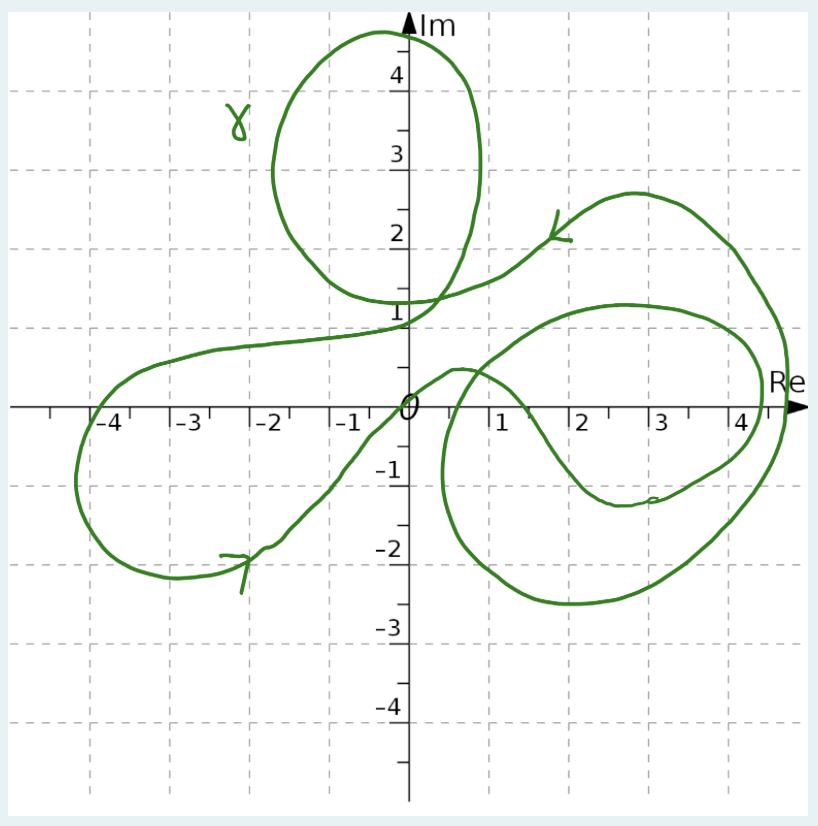
\includegraphics[width=0.58\textwidth]{assets/chapter2/kurve_aufgabe5_2024.png}
\end{center}

\textbf{Schritt 1: Singularitäten und relevante Teilintegrale.}
Der erste Summand hat bei $2$ einen Pol zweiter Ordnung. Der zweite Summand hat
einfache Pole bei $\pm3\ii$; wegen $\wind(\gamma,-3\ii)=0$ trägt $-3\ii$ nichts
bei. Wir setzen
\[
I_1=\int_{\gamma_2}\frac{\cos z}{(z-2)^2}\dd z,
\qquad
I_2=\int_{\gamma_{3\ii}}\frac{\ee^z}{z^2+9}\dd z,
\]
wobei $\gamma_w(t)=w+\ee^{2\pi\ii t}$ jeweils einmal positiv um $w$ läuft. Dann
\[
I=2I_1-I_2.
\]

\textbf{Schritt 2: Pol zweiter Ordnung mit der Ableitungsformel.}
\[
I_1
=2\pi\ii\,(\cos z)'\big|_{z=2}
=-2\pi\ii\sin2.
\]

\textbf{Schritt 3: Einfacher Pol bei $3\ii$.}
Wir schreiben
\[
\frac{\ee^z}{z^2+9}
=\frac{1}{z-3\ii}\,\frac{\ee^z}{z+3\ii}.
\]
Der zweite Faktor ist bei $3\ii$ holomorph. Daher
\[
I_2
=2\pi\ii\left.\frac{\ee^z}{z+3\ii}\right|_{z=3\ii}
=2\pi\ii\frac{\ee^{3\ii}}{6\ii}
=\frac{\pi}{3}\ee^{3\ii}.
\]

\textbf{Schritt 4: Windungszahlen einsetzen.}
\[
\boxed{
I=2(-2\pi\ii\sin2)-\frac{\pi}{3}\ee^{3\ii}
=-4\pi\ii\sin2-\frac{\pi}{3}\ee^{3\ii}
}.
\]
\end{beispielbox}

\begin{trainingsbox}[title=Trainingsaufgabe: verschiedene Kurven]
Gegeben sei
\[
f(z)=\frac1z\,\frac1{z+1}
=\frac1z-\frac1{z+1}.
\]
Bestimmen Sie für jede der drei dargestellten Kurven den Wert von
$\int_\gamma f(z)\dd z$. Pfeile geben die jeweilige Orientierung an.

\begin{center}
\begin{minipage}{0.31\textwidth}
\centering
\textbf{Kurve 1}\\[1mm]
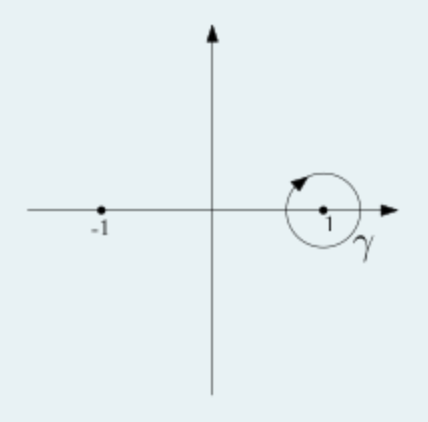
\includegraphics[width=\linewidth]{assets/chapter2/kurve_training_1.png}
\end{minipage}
\begin{minipage}{0.31\textwidth}
\centering
\textbf{Kurve 2}\\[1mm]
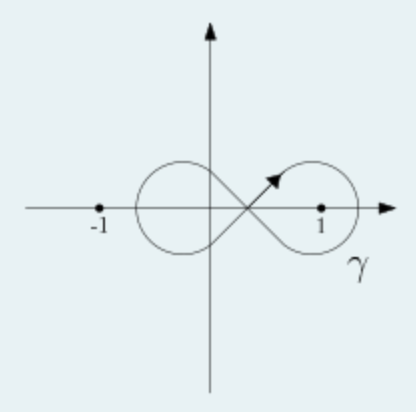
\includegraphics[width=\linewidth]{assets/chapter2/kurve_training_2.png}
\end{minipage}
\begin{minipage}{0.31\textwidth}
\centering
\textbf{Kurve 3}\\[1mm]
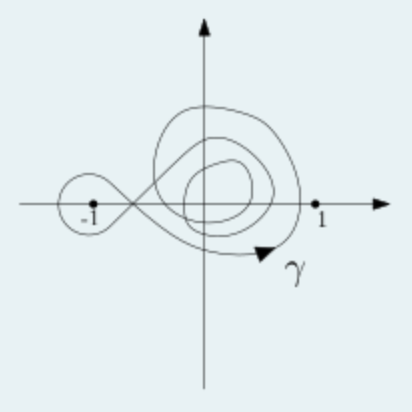
\includegraphics[width=\linewidth]{assets/chapter2/kurve_training_3.png}
\end{minipage}
\end{center}

\textbf{Auswahlmöglichkeiten:}
\[
0,\qquad 2\pi\ii,\qquad4\pi\ii,\qquad-2\pi\ii,\qquad8\pi\ii.
\]
\end{trainingsbox}
\kariert[7cm]

\subsection{Mittelwertsatz, Maximumprinzip und Liouville}
\begin{satzbox}[title=Mittelwertsatz]
Ist $f$ auf einer Umgebung der abgeschlossenen Kreisscheibe
$\overline{B(z_0,r)}$ holomorph, dann
\[
f(z_0)=\frac1{2\pi}\int_0^{2\pi}f(z_0+r\ee^{\ii t})\dd t.
\]
\end{satzbox}

\begin{satzbox}[title=Maximum-Modulus-Prinzip]
Eine nichtkonstante holomorphe Funktion auf einem Gebiet besitzt im Inneren kein
Maximum ihres Betrags. Ist $f$ auf einem kompakten Gebiet stetig und im Inneren
holomorph, so wird $\max|f|$ am Rand angenommen.
\end{satzbox}

\begin{satzbox}[title=Satz von Liouville]
Jede beschränkte ganze Funktion ist konstant.
\end{satzbox}

Nützliche Varianten folgen durch geschicktes Transformieren. Ist etwa
$|\Ree f(z)|\le C$ für eine ganze Funktion $f$, dann ist $\ee^{f(z)}$ beschränkt,
denn $|\ee^{f(z)}|=\ee^{\Ree f(z)}\le\ee^C$. Nach Liouville ist $\ee^f$
konstant; daraus folgt auch, dass $f$ konstant ist.

\begin{mcbox}[title=MC-Training: Liouville und ganze Funktionen]
Sei $f:\C\to\C$ holomorph. Entscheiden Sie für jede Aussage, ob sie immer wahr
oder falsch ist.
\begin{enumerate}
\item Falls $g:\C\to\C$ holomorph ist und
\[
|g(z)|<|f(z)|\qquad\text{für alle }z\in\C,
\]
so gibt es eine Konstante $\lambda\in\C$ mit
$g(z)=\lambda f(z)$ für alle $z\in\C$.
\[
\square\ \text{Wahr}\qquad\qquad\square\ \text{Falsch}
\]

\item Falls $|f(z)|\le|f'(z)|$ für alle $z\in\C$, so ist $f$ konstant.
\[
\square\ \text{Wahr}\qquad\qquad\square\ \text{Falsch}
\]

\item Falls es ein $C\in\R$ mit
\[
|\Ree f(z)|\le C\qquad\text{für alle }z\in\C
\]
gibt, so gibt es ein $C'>0$ mit $|f(z)|\le C'$ für alle $z\in\C$.
\[
\square\ \text{Wahr}\qquad\qquad\square\ \text{Falsch}
\]

\item Falls es ein $C\in\R$ mit $|f(z)|\le C$ für alle $z\in\C$ gibt, so
gibt es ein $C'>0$ mit $|\Ree f(z)|\le C'$ für alle $z\in\C$.
\[
\square\ \text{Wahr}\qquad\qquad\square\ \text{Falsch}
\]
\end{enumerate}
\end{mcbox}

\begin{pruefungsbox}
\begin{itemize}
\item Beim Maximumprinzip muss zwischen einem offenen Gebiet und seinem kompakten
Abschluss unterschieden werden.
\item Vor Cauchy stets prüfen: Welche Nennernullstellen liegen innen? 
\item Systematisch das Kochrezept abarbeiten, in angepassten Aufgabenstellungen können Schritte übersprungen werden.
\end{itemize}
\end{pruefungsbox}
}

\ThemeTwo
\ThemeThree
\ThemeFour
\ThemeFive
\ThemeSix
\FinalStrategy

\end{document}
